%---------------------------------------------------------------------
\begin{frame}{Welcome to EC 387!}

    \begin{itemize}
        \item Class \newbold{objectives}
        \begin{itemize}
            \item Show you real-world applications of economic theory concepts in the context of healthcare
            \item Teach you how to analyze current issues in health and healthcare through the lens of economics
        \end{itemize}
        \vspace{3mm}

        \item Difficulty: moderate
        \begin{itemize}
            \item You will be asked to solve numerical and graphical problems
            \item You will also be asked to determine what economic models and graphical frameworks apply to the problem at hands
        \end{itemize}
    \end{itemize}
\end{frame}
%---------------------------------------------------------------------
\begin{frame}{Why is learning about health economics important?}

    \begin{itemize}
        \item What I want this class to bring you
        \begin{itemize}
            \item An understanding of core economic theories applied to healthcare
            \item An opportunity to familiarize yourself with the U.S. healthcare system and U.S. healthcare policy
            \item Allow you to analyze current and future healthcare policy debates
            \item Help you build confidence to act as an economic thinker in the future
        \end{itemize}
        \vspace{3mm}

        \item How can this be helpful in your life?
        \begin{itemize}
            \item Help prepare you for healthcare related jobs (healthcare providers, lawyers, management and economic consultants, software developpers, etc.)
            \item Help you become more informed healthcare consumers
            \item Prepare you to better understand healthcare news and debates
        \end{itemize}
        \vspace{3mm}
    \end{itemize}
    \only<1>{\vspace{5mm}}
    \only<2>{$\implies$ \textit{Why did \newbold{you} choose to take this class?}}

\end{frame}
%---------------------------------------------------------------------
\begin{frame}{About me}

    \begin{itemize}
        \item I am a tenure-track assistant professor in the Economics Department at BU
        \begin{itemize}
            \item I spend a lot of time on research, specializing in the organization of production in healthcare markets
            \item Some of my work:
            \begin{itemize}
                \item Where are healthcare services \textit{produced} and \textit{consumed} in the U.S.? {\small \textcolor{maroon}{Dingel, Gottlieb, Lozinski, Mourot (2024)}}
                \item Should top surgeons practice at top hospitals? {\small \textcolor{maroon}{Mourot (2025)}}
            \end{itemize}
        \end{itemize}
        \vspace{3mm}
        % Most of my time on research and writing papers on the organization of healthcare markets
        % I have studied the allocation of healthcare across space: DGLM
        % I have studied how surgeons and hospitals interact in the production of survival in surgery

        \item I have worked in economic consulting before my PhD, specializing in \newbold{Antitrust}
    \end{itemize}
\end{frame}
%---------------------------------------------------------------------
\begin{frame}{}

    {\Large \textcolor{maroon}{Some facts we will study in this course}}

\end{frame}
%---------------------------------------------------------------------
\begin{frame}{We spend more and more per capita on healthcare...}

    \begin{center}
        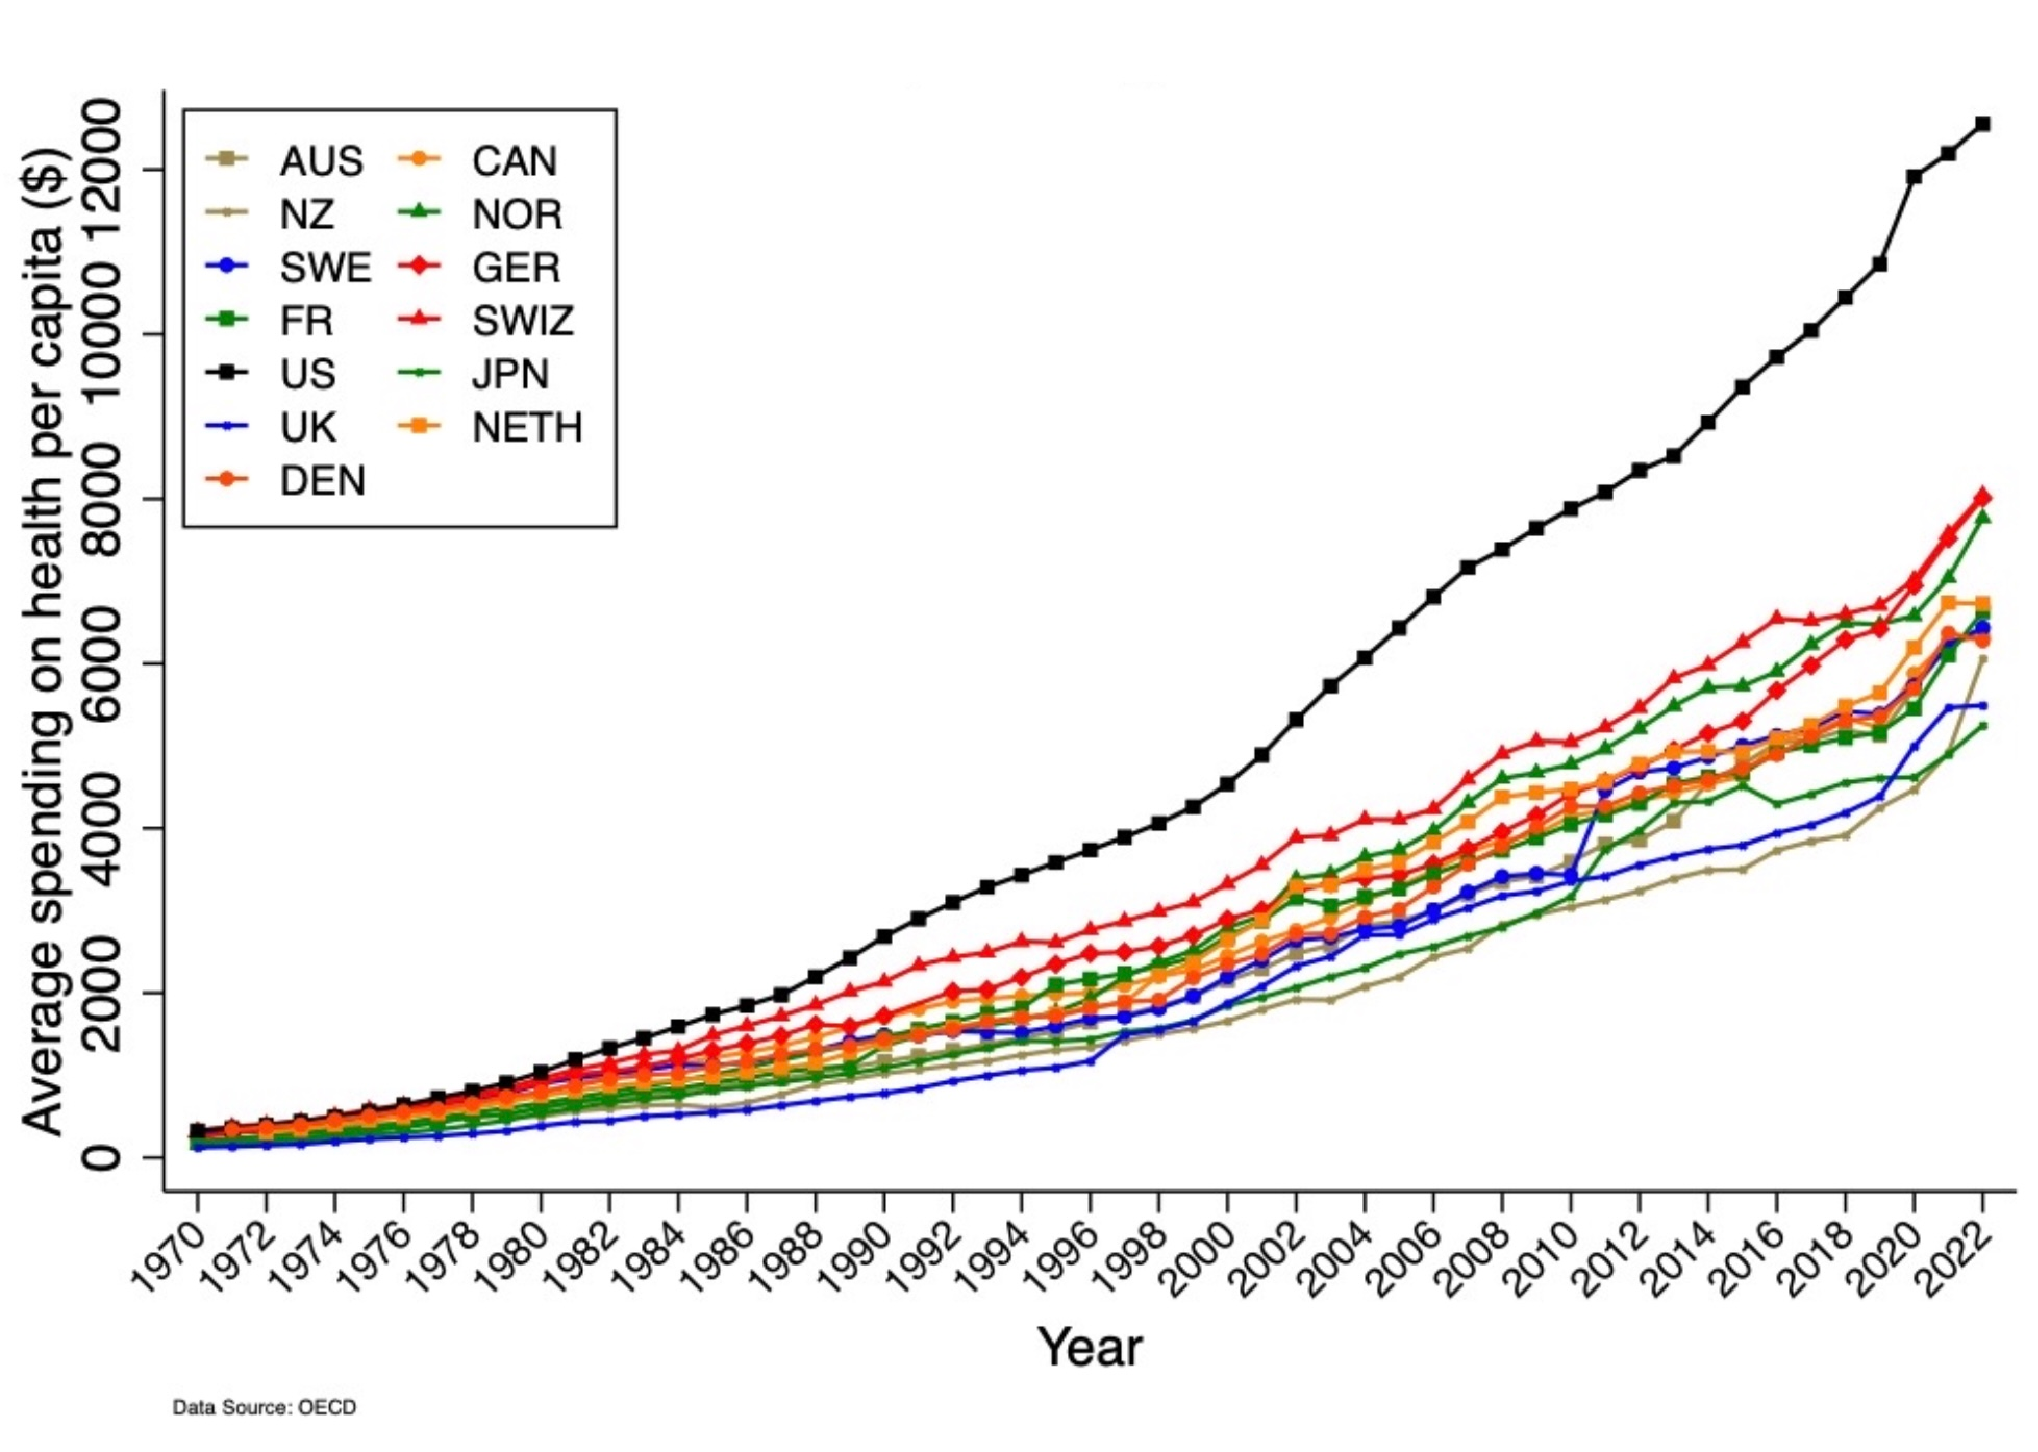
\includegraphics[height=0.85\textheight]{input/oecd_spendingpc.pdf}
    \end{center}

\end{frame}
%---------------------------------------------------------------------
\begin{frame}{... And also as a share of GDP...}

    \begin{center}
        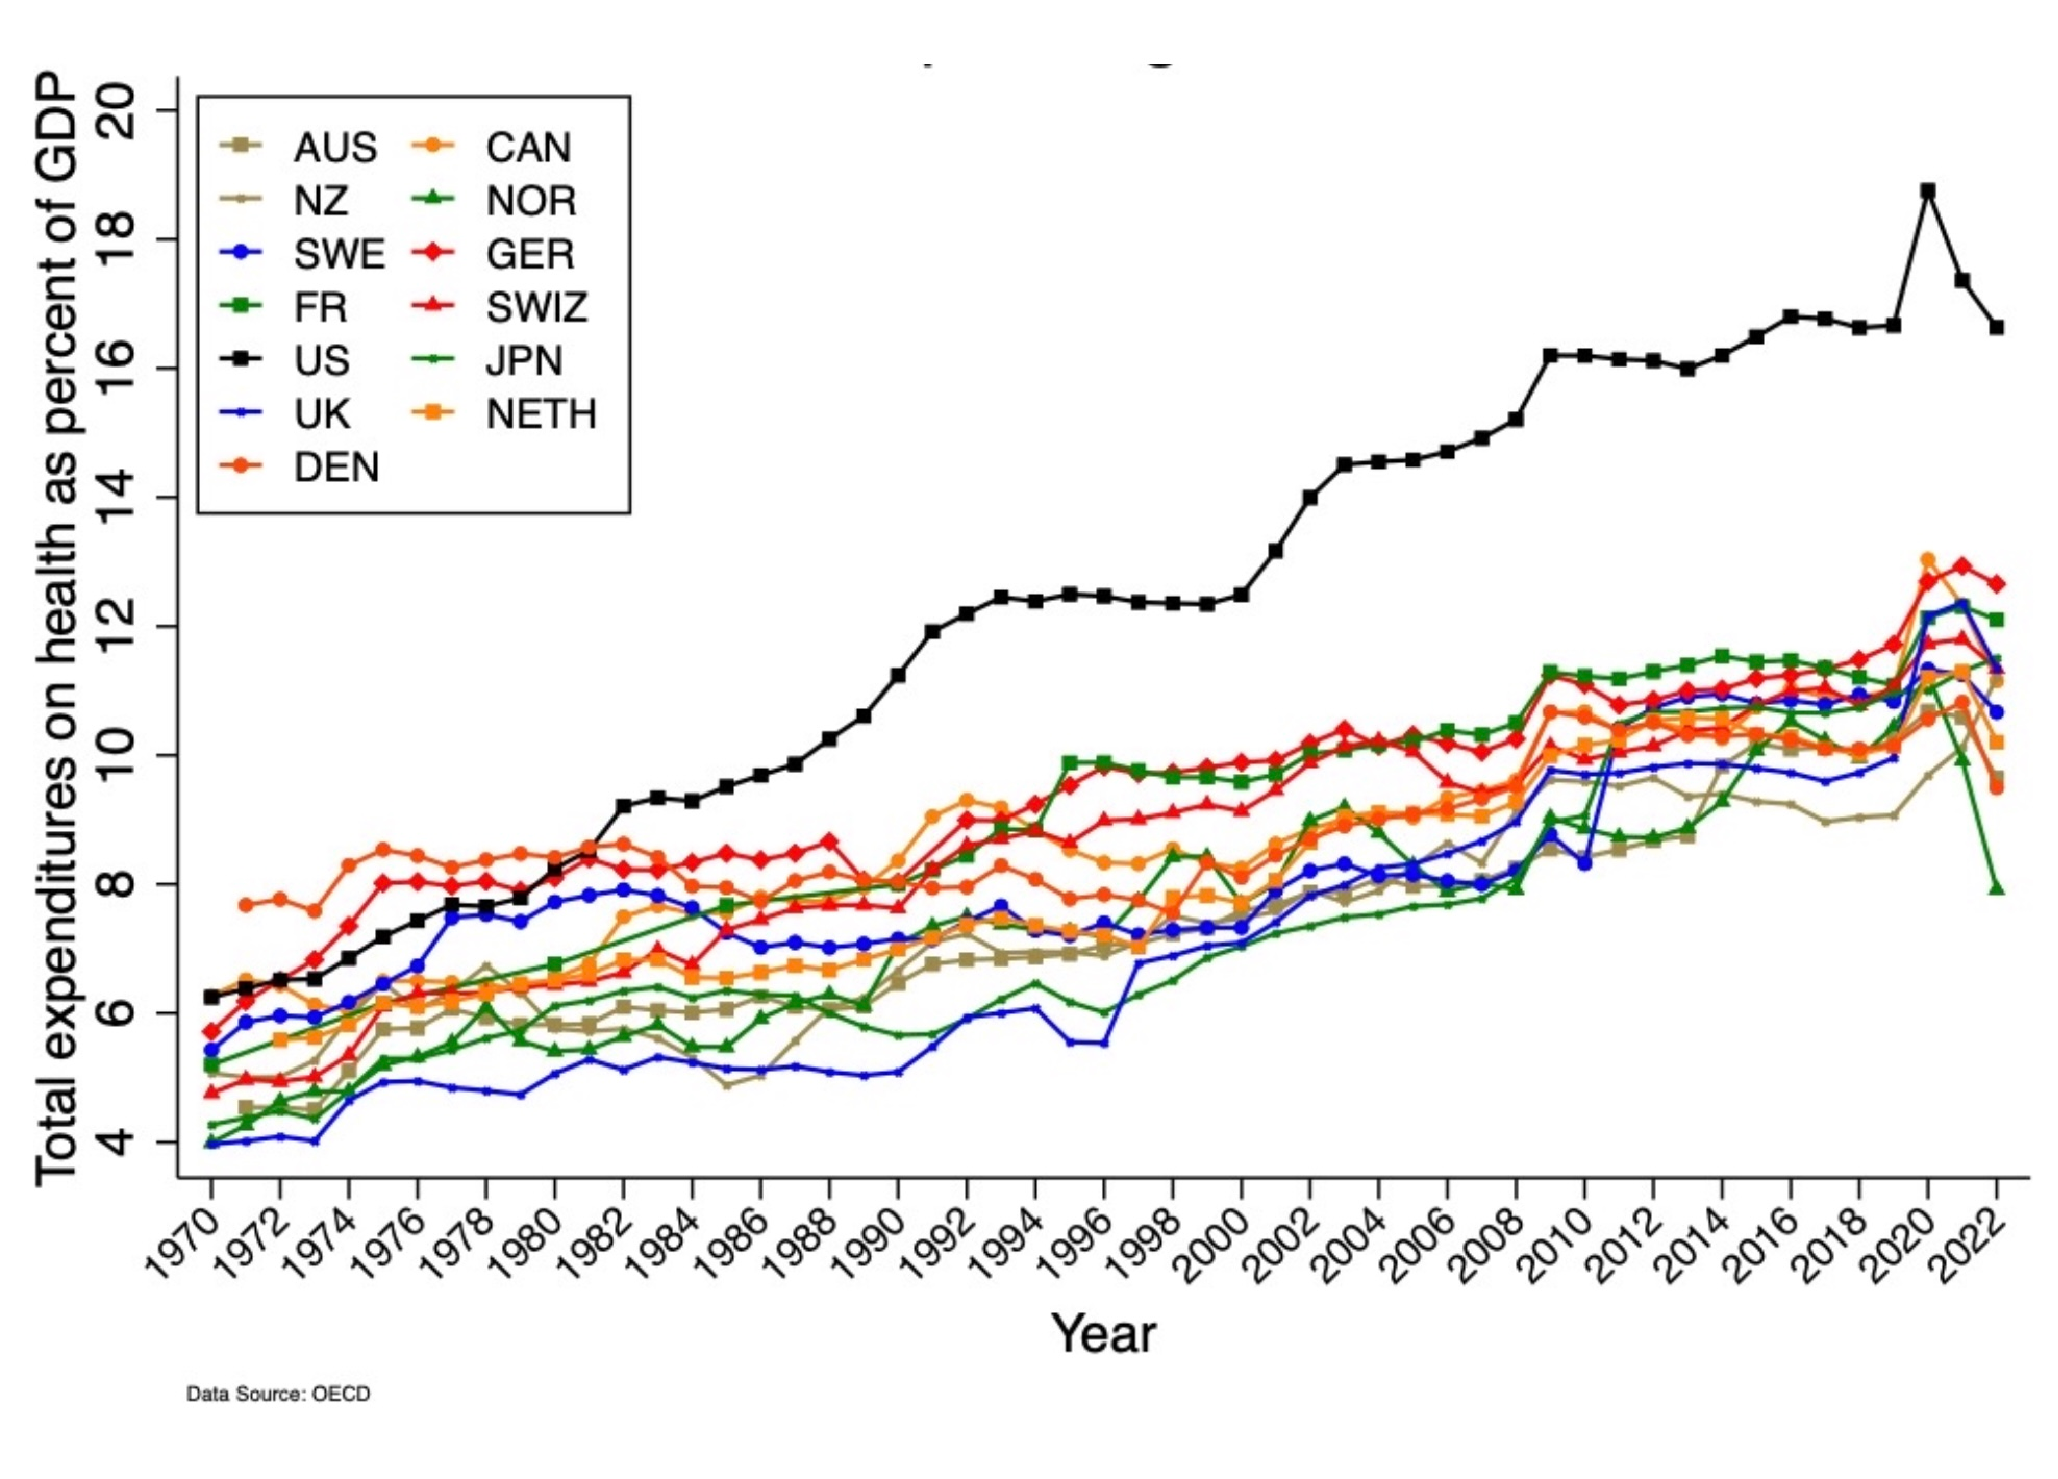
\includegraphics[height=0.85\textheight]{input/oecd_spendinggdp.pdf}
    \end{center}

\end{frame}
%---------------------------------------------------------------------
\begin{frame}{... Yet mixed returns on longevity in the U.S.}

    \begin{center}
        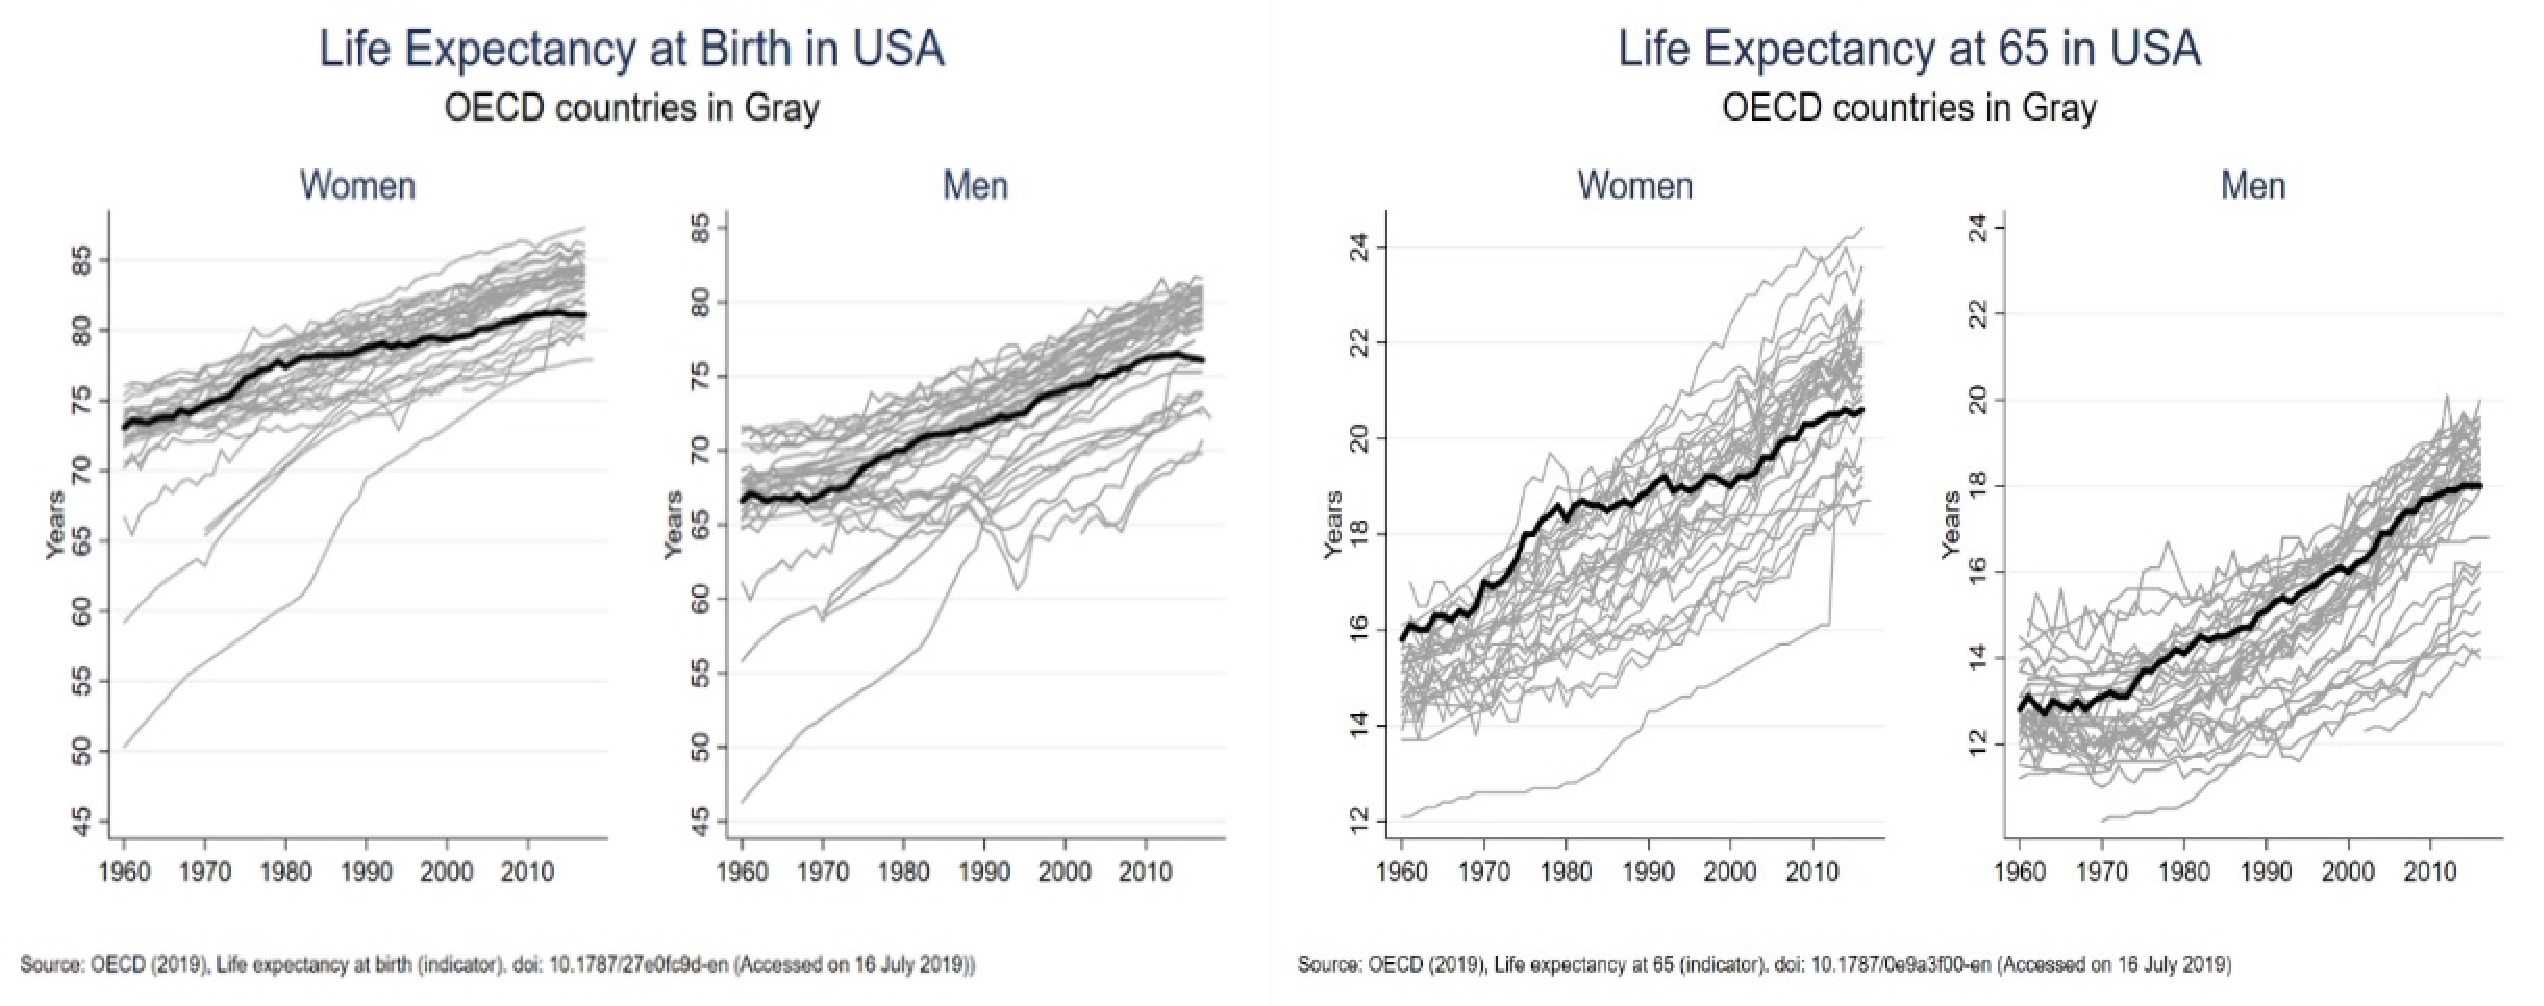
\includegraphics[height=0.7\textheight]{input/oecd_lifeexpectancy.pdf}
    \end{center}
\end{frame}
%---------------------------------------------------------------------
\begin{frame}{Spending varies a lot across regions in the U.S.}

    \only<1>{
        \begin{center}
            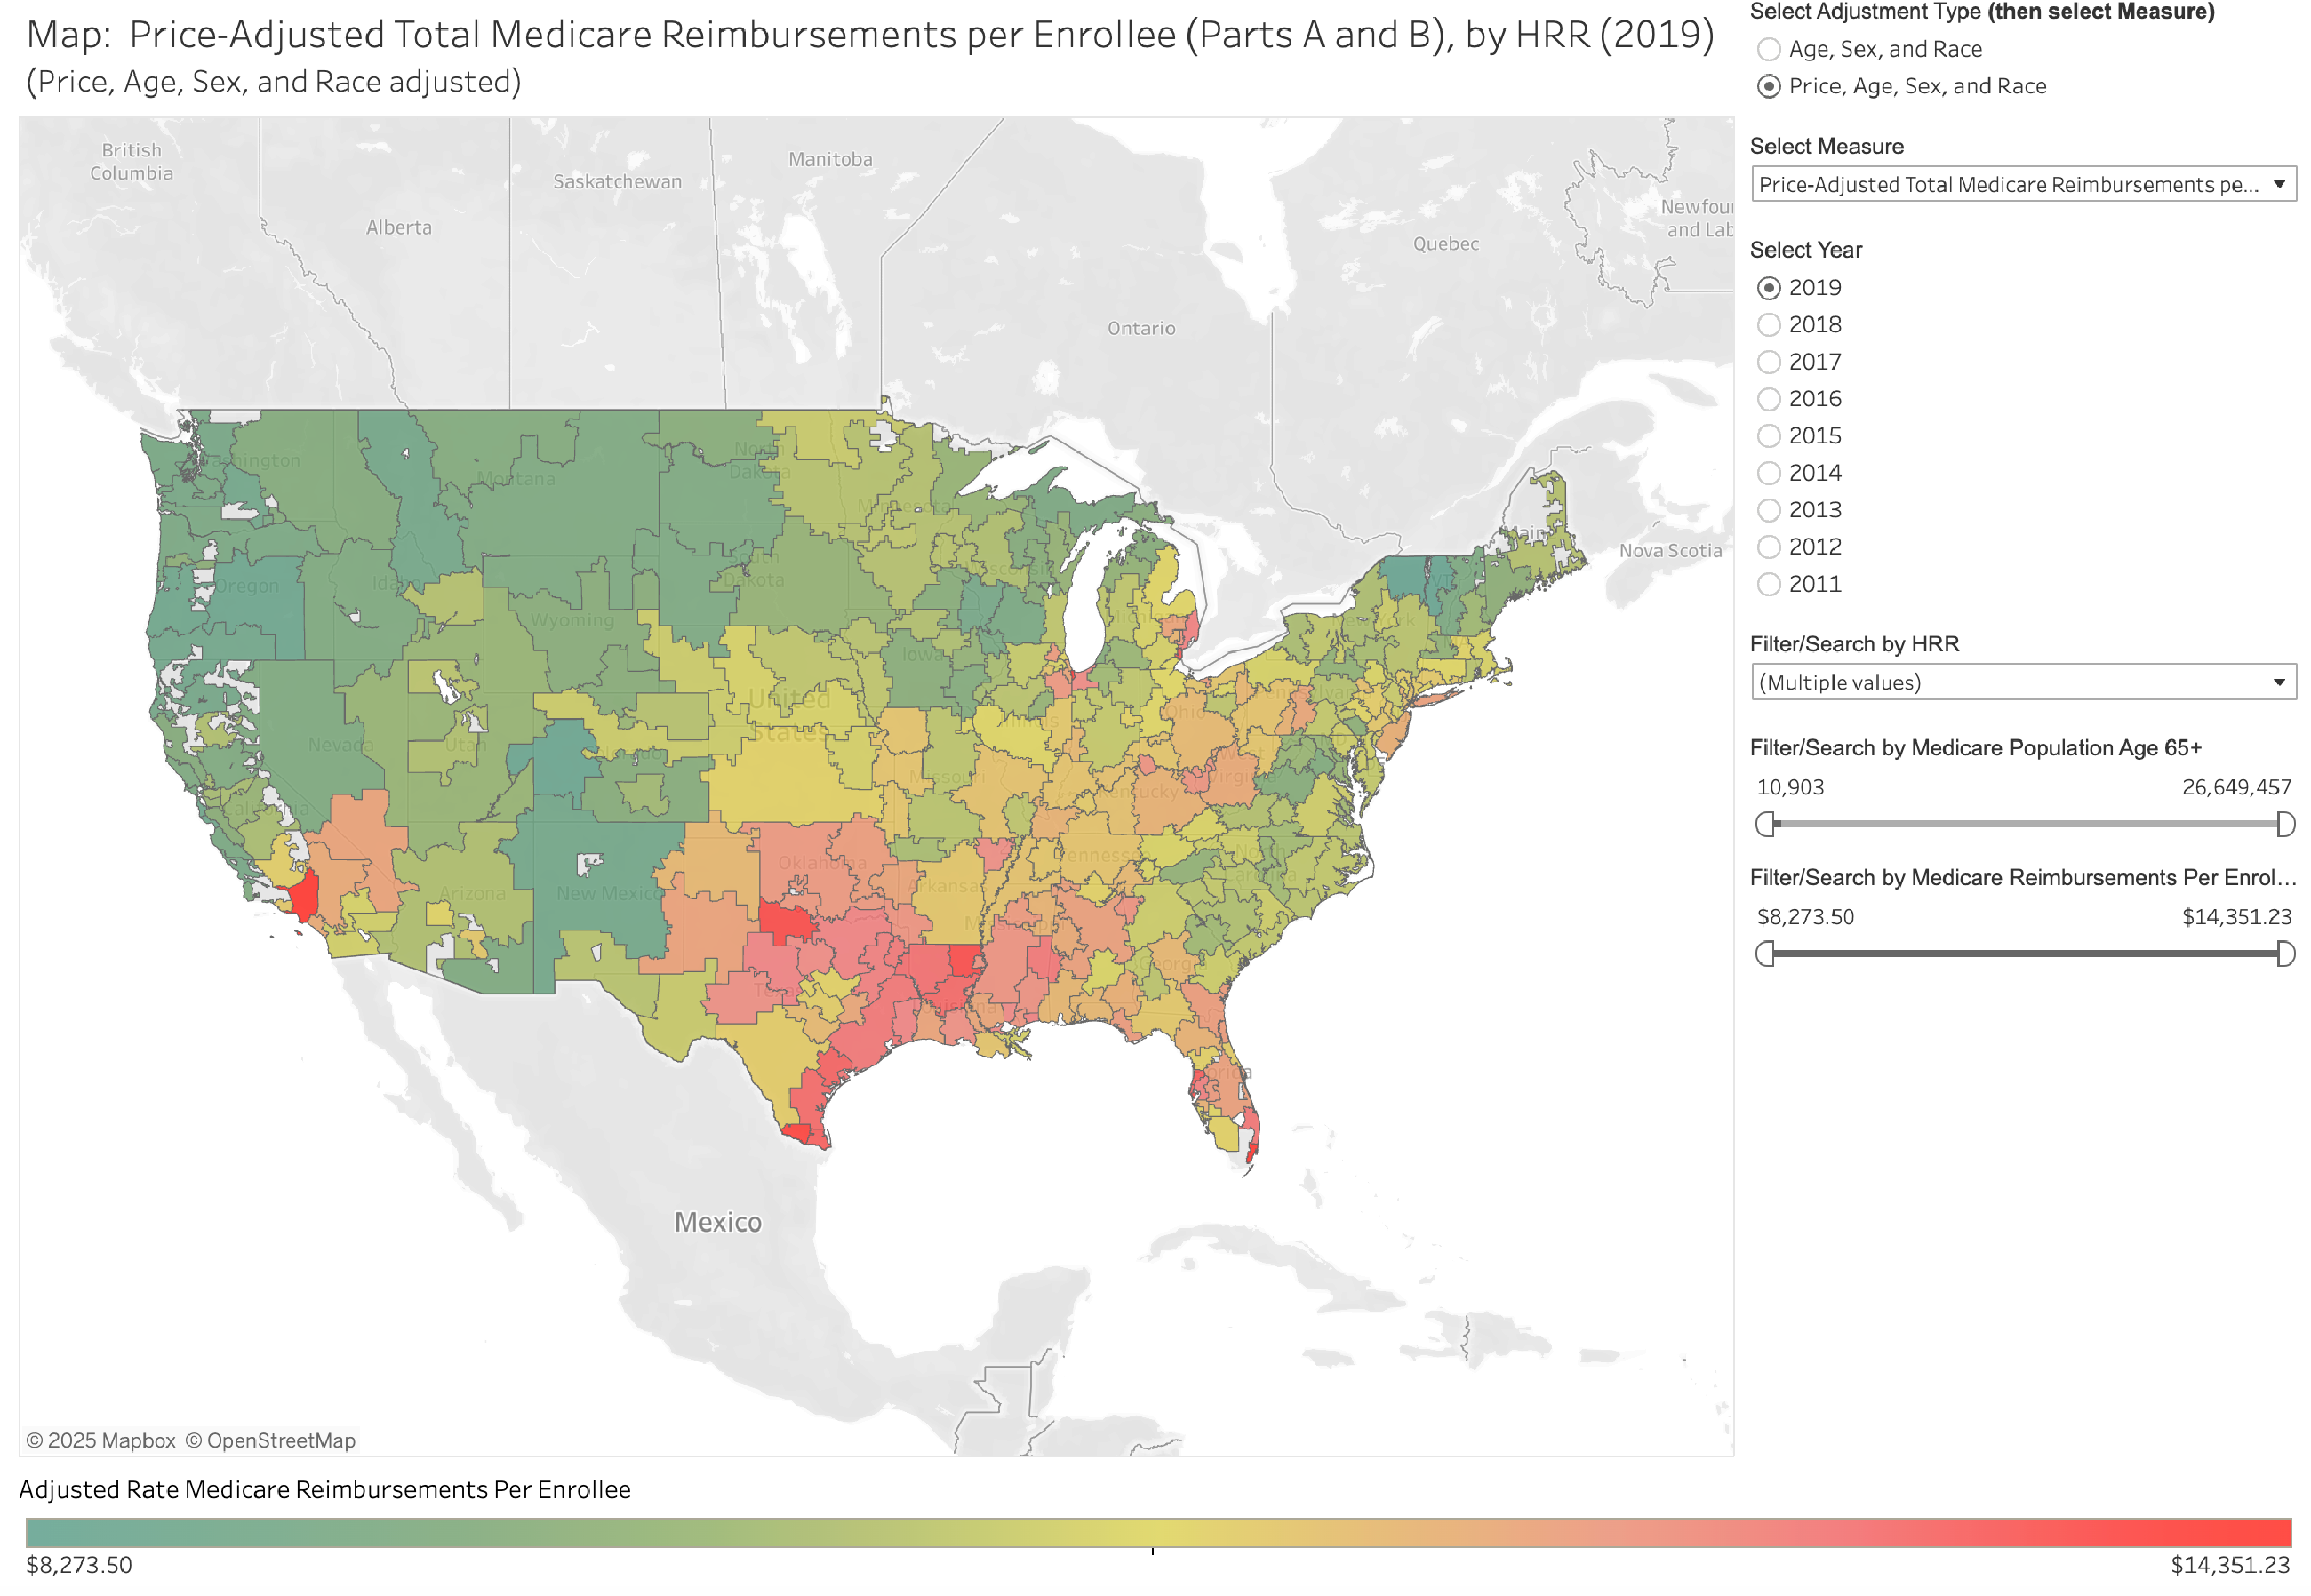
\includegraphics[height=0.85\textheight]{input/dartmouth_map_reimbursement.pdf}
        \end{center}
    }
    \only<2>{
        \begin{center}
            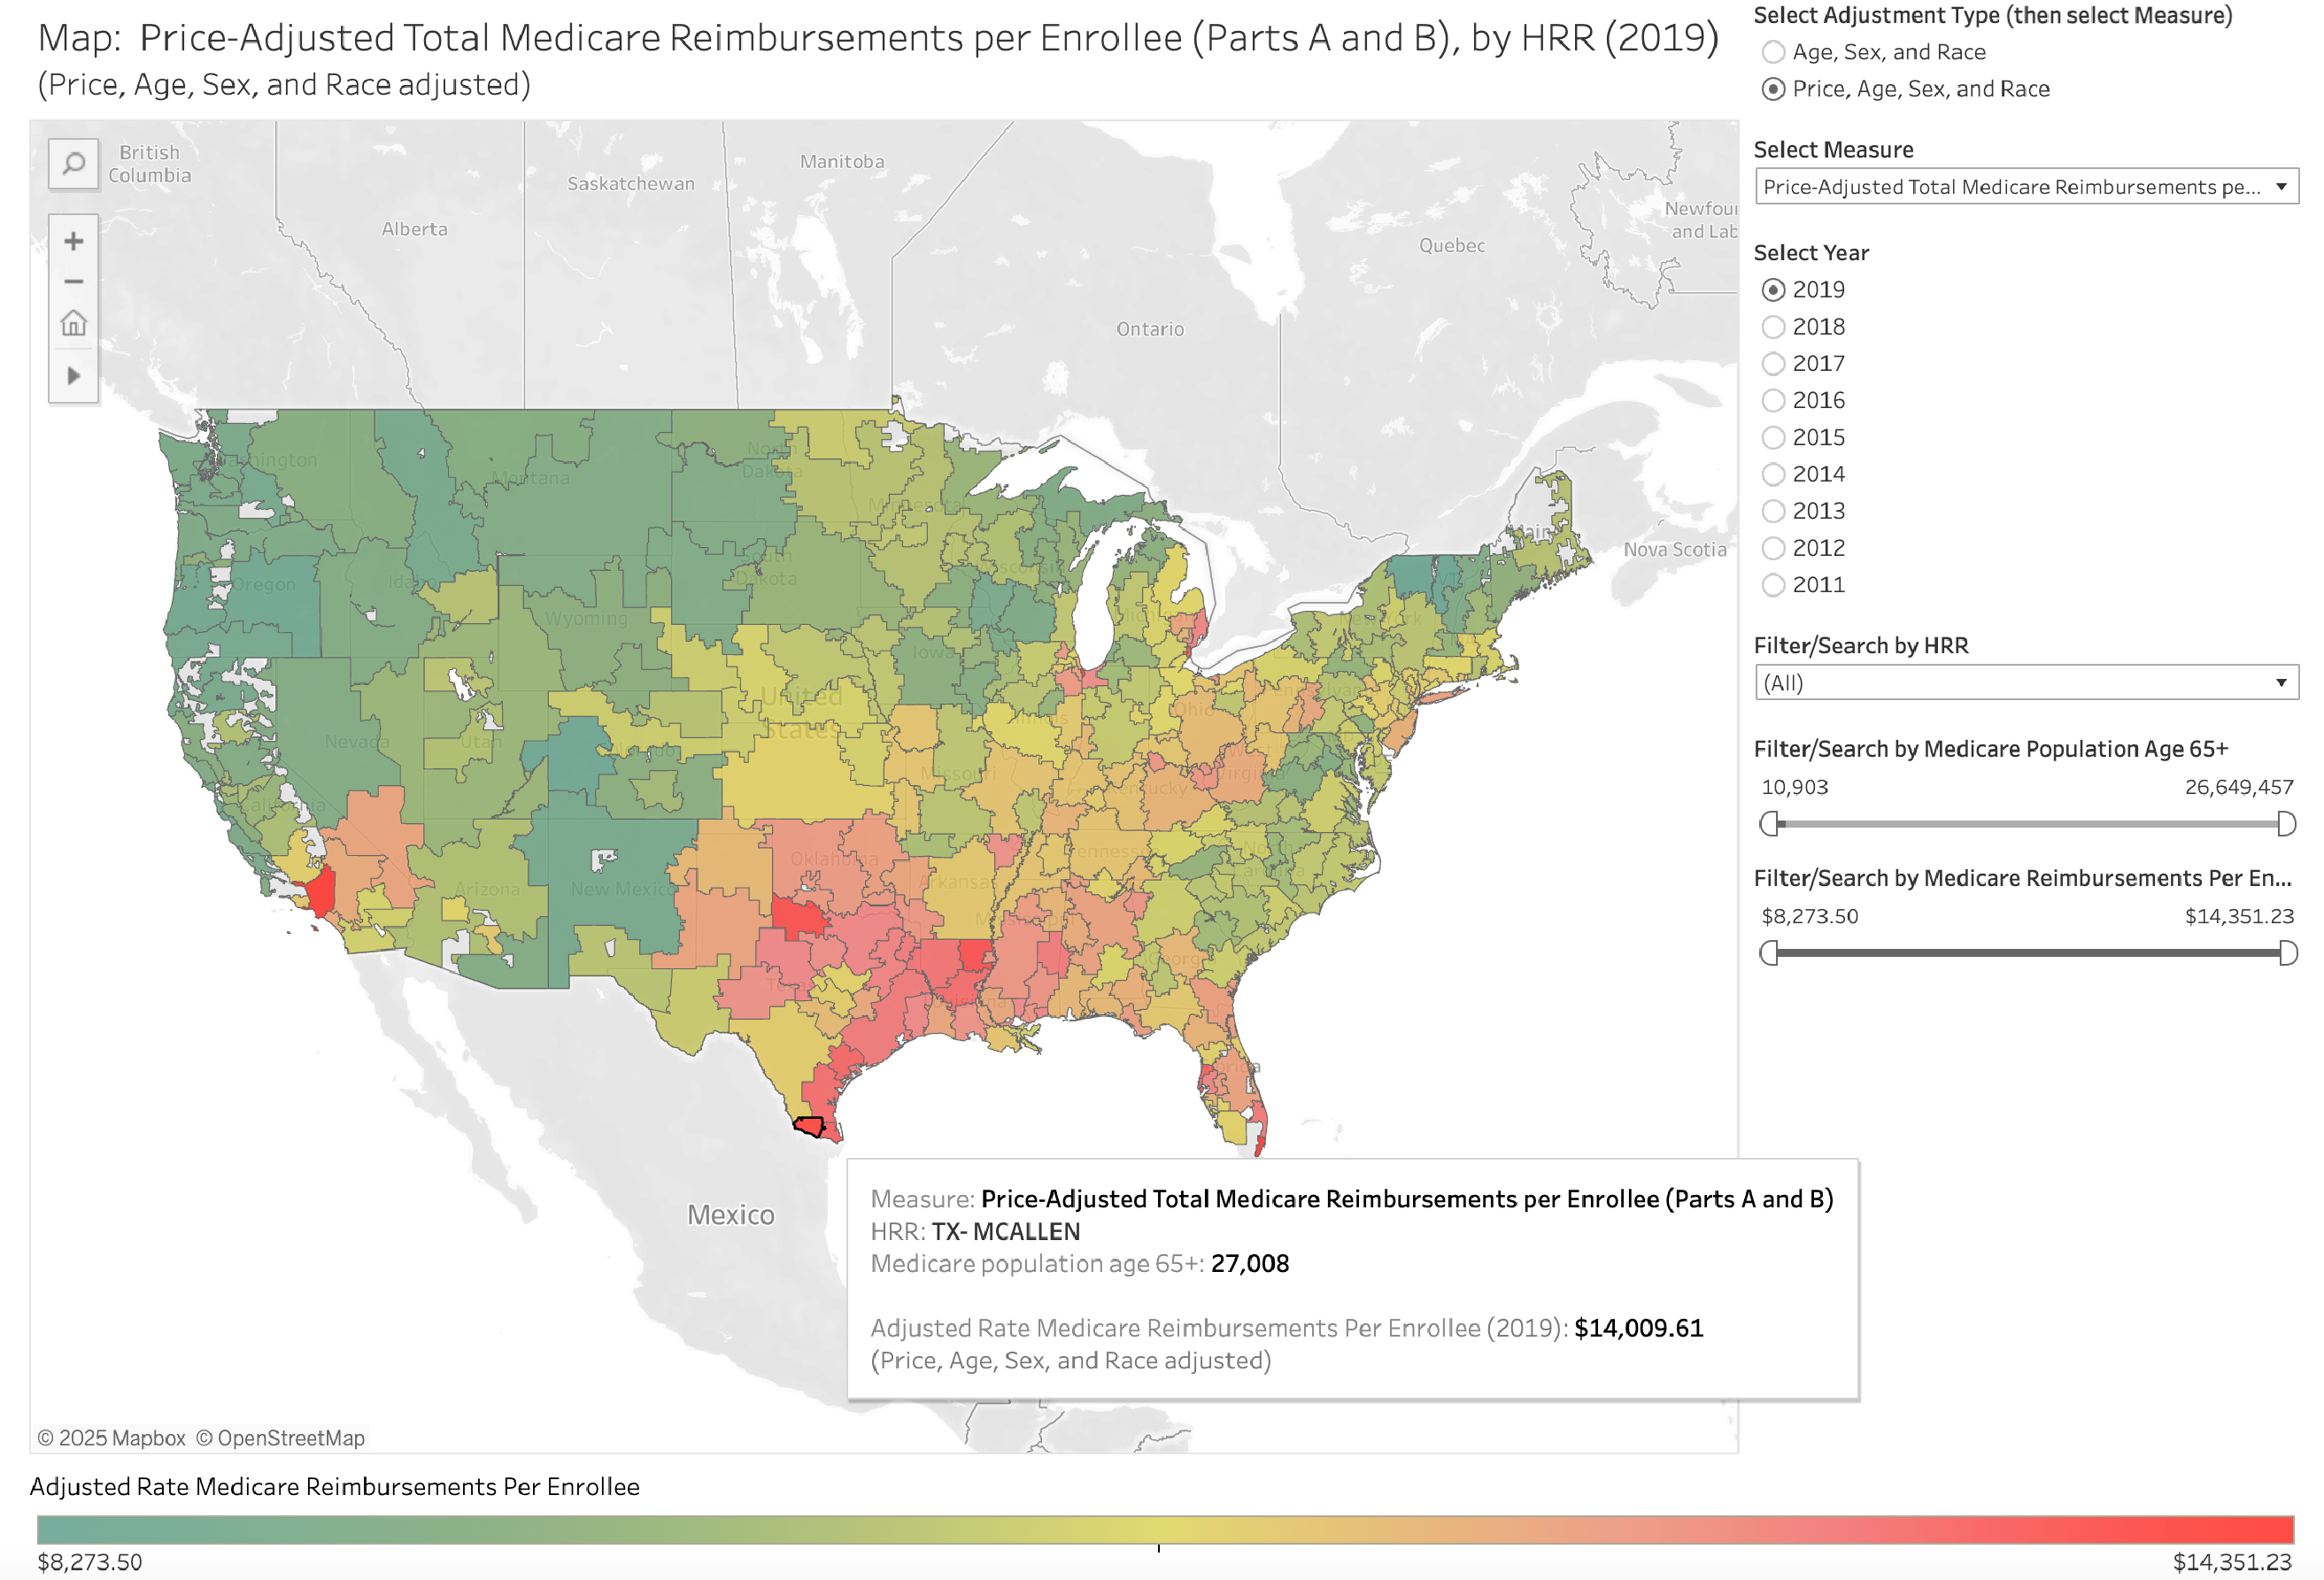
\includegraphics[height=0.85\textheight]{input/dartmouth_map_reimbursement_McAllen.pdf}
        \end{center}
    }
    \only<3>{
        \begin{center}
            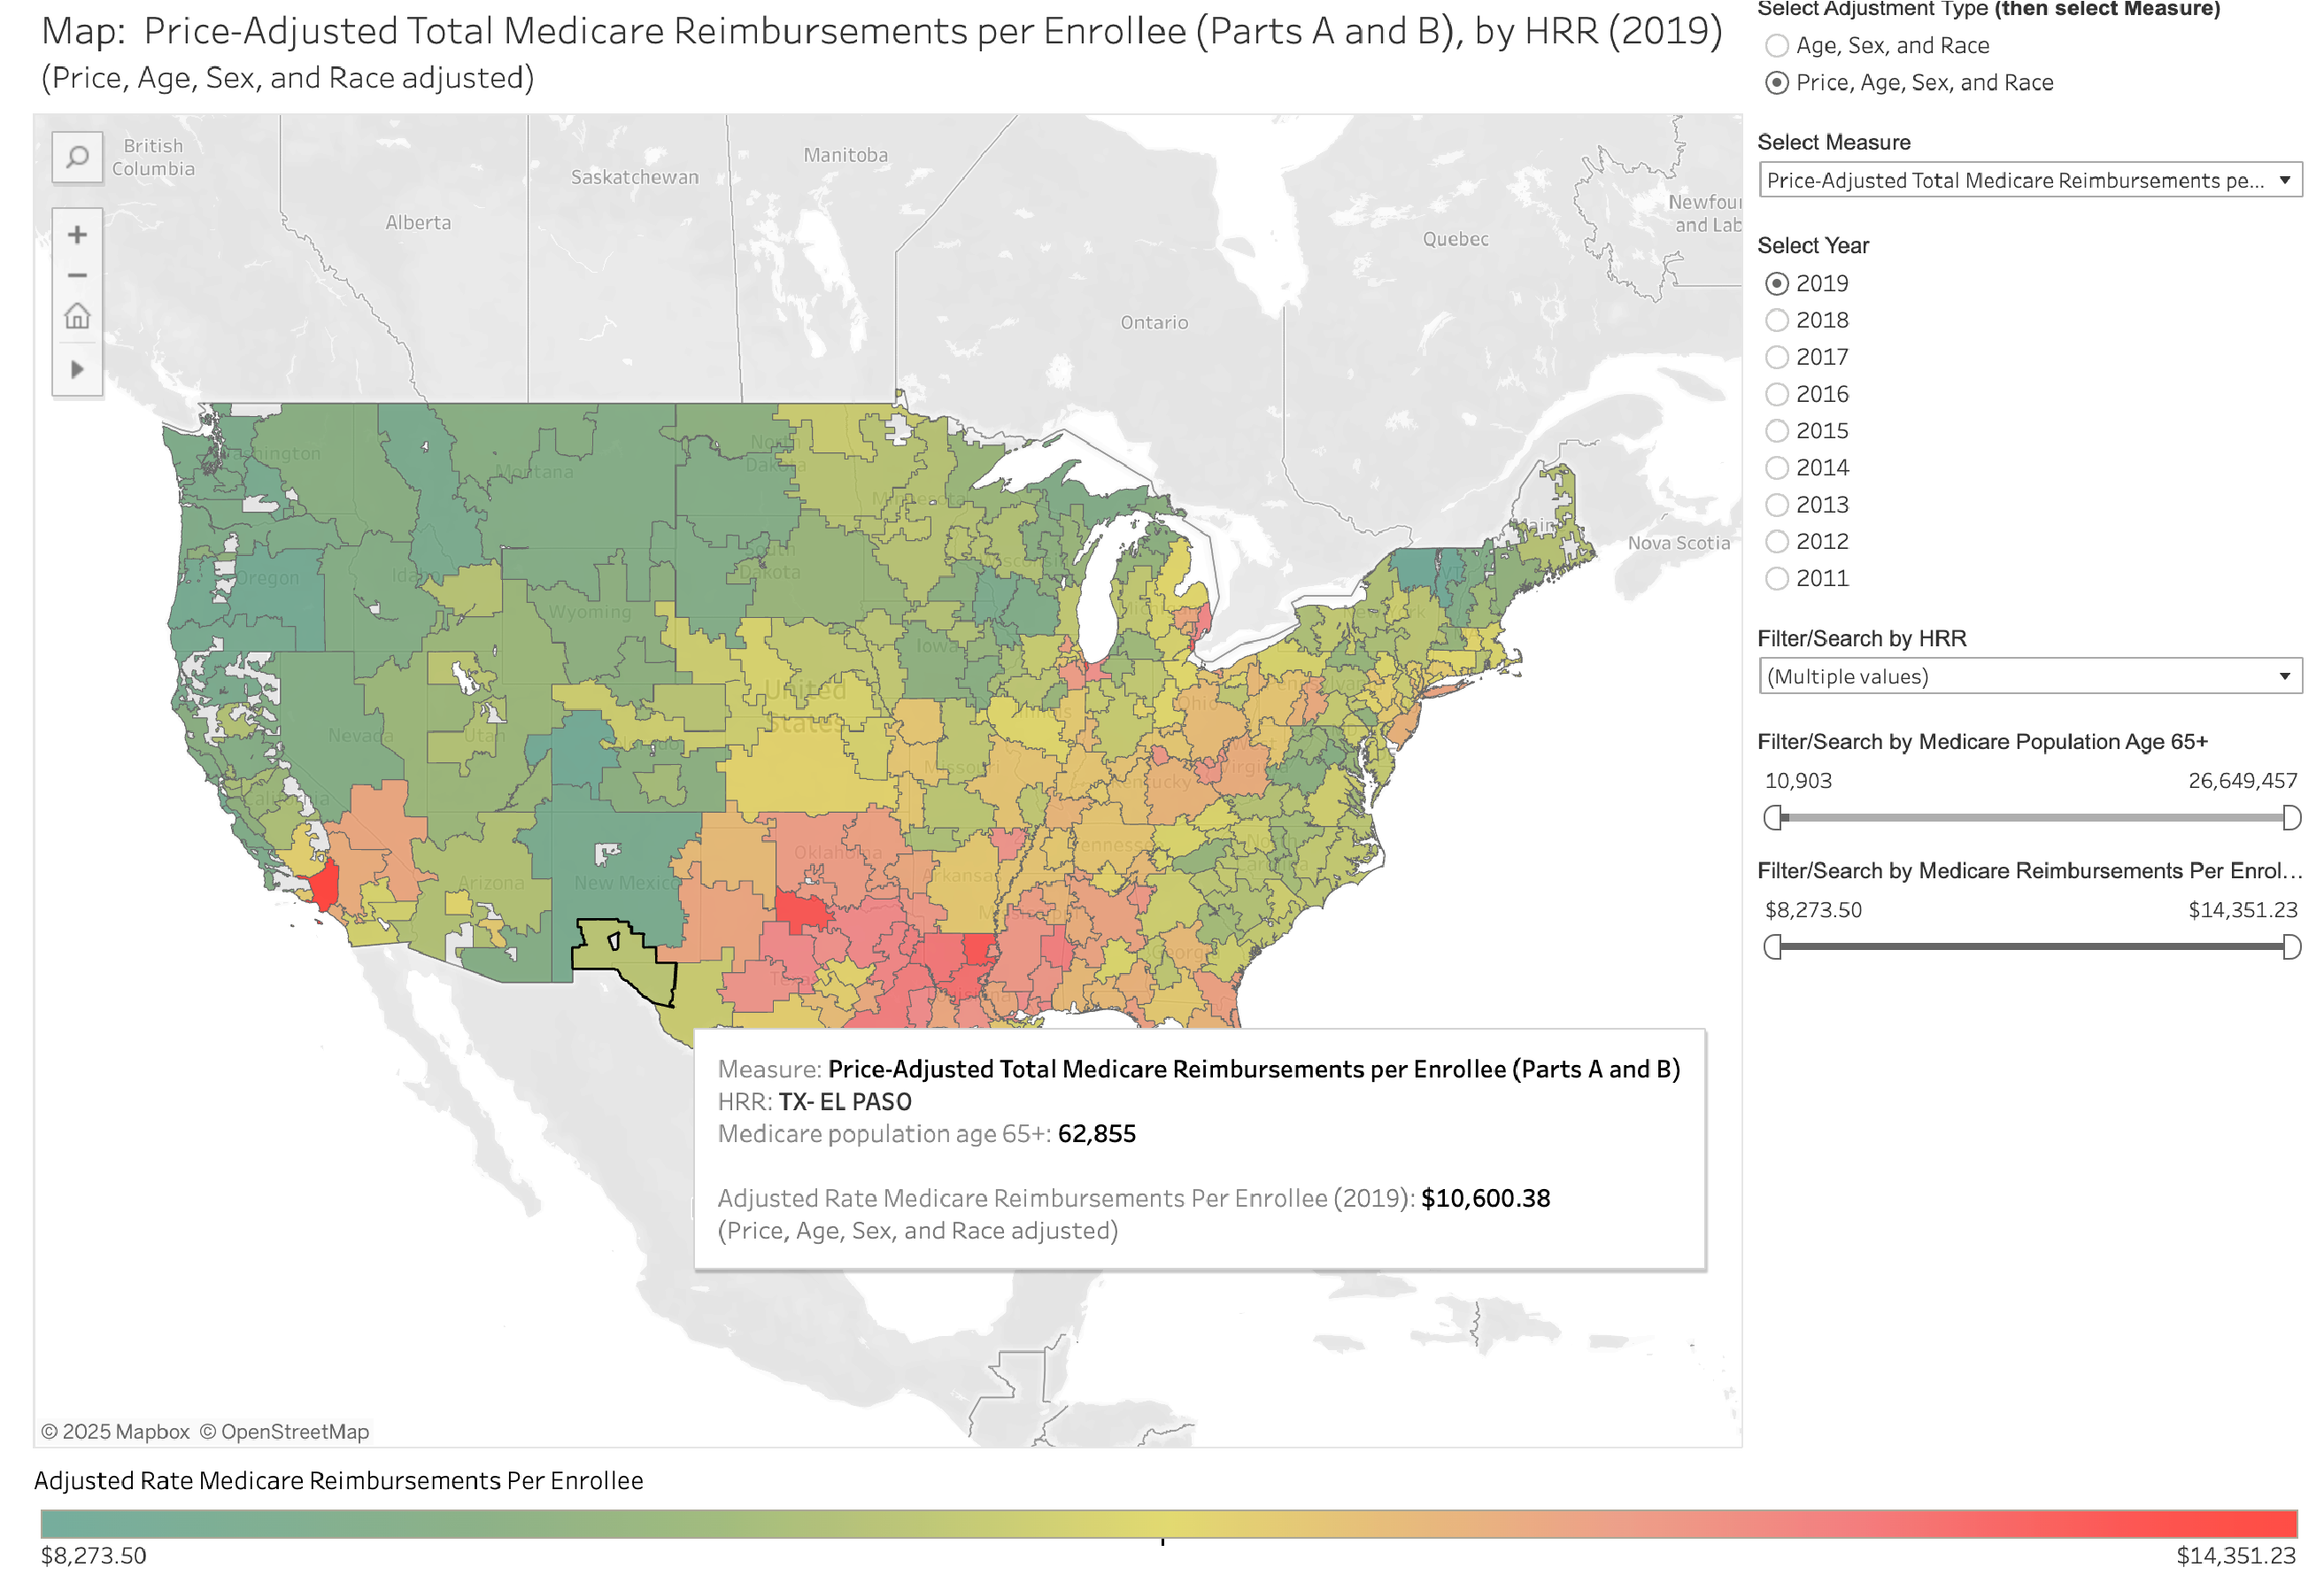
\includegraphics[height=0.85\textheight]{input/dartmouth_map_reimbursement_Elpaso.pdf}
        \end{center}
    }
    \vspace{-3mm}
  
    {\scriptsize From Dartmouth Atlas Project \href{https://www.dartmouthatlas.org/interactive-apps/medicare-reimbursements/}{\underline{website}}.}
  
\end{frame}
%---------------------------------------------------------------------
\begin{frame}{Patients respond to financial incentives...}

    \begin{center}
        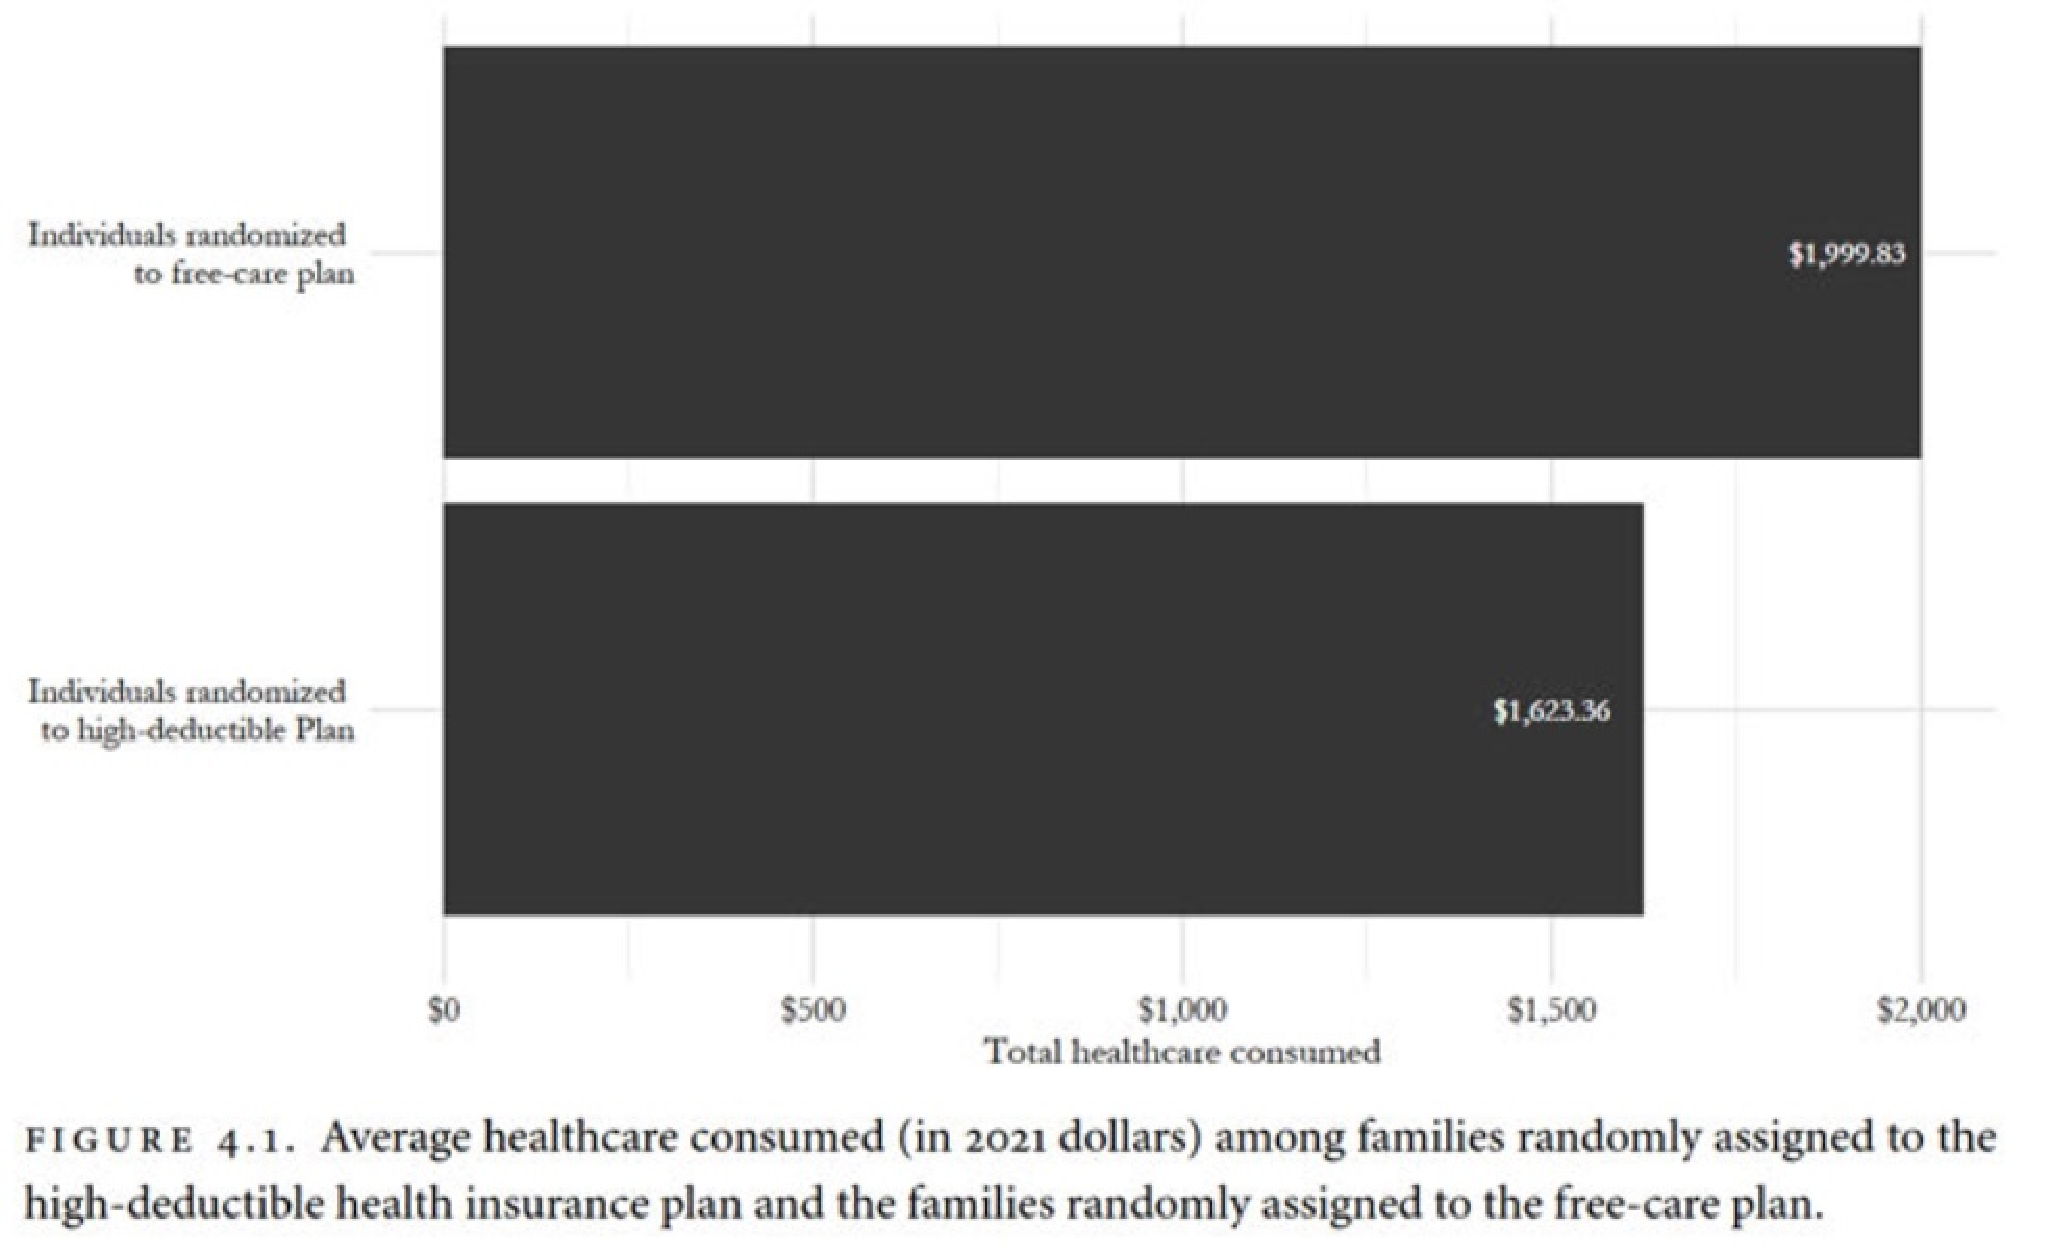
\includegraphics[height=0.75\textheight]{input/GrossNoto_fig4_1.pdf}
    \end{center}

    {\tiny Source: \textit{Better Health Economics} by Tal Gross and Matthew Notowidigdo, chapter 4.}

\end{frame}
%---------------------------------------------------------------------
\begin{frame}{... and physicians too!}

    \begin{center}
        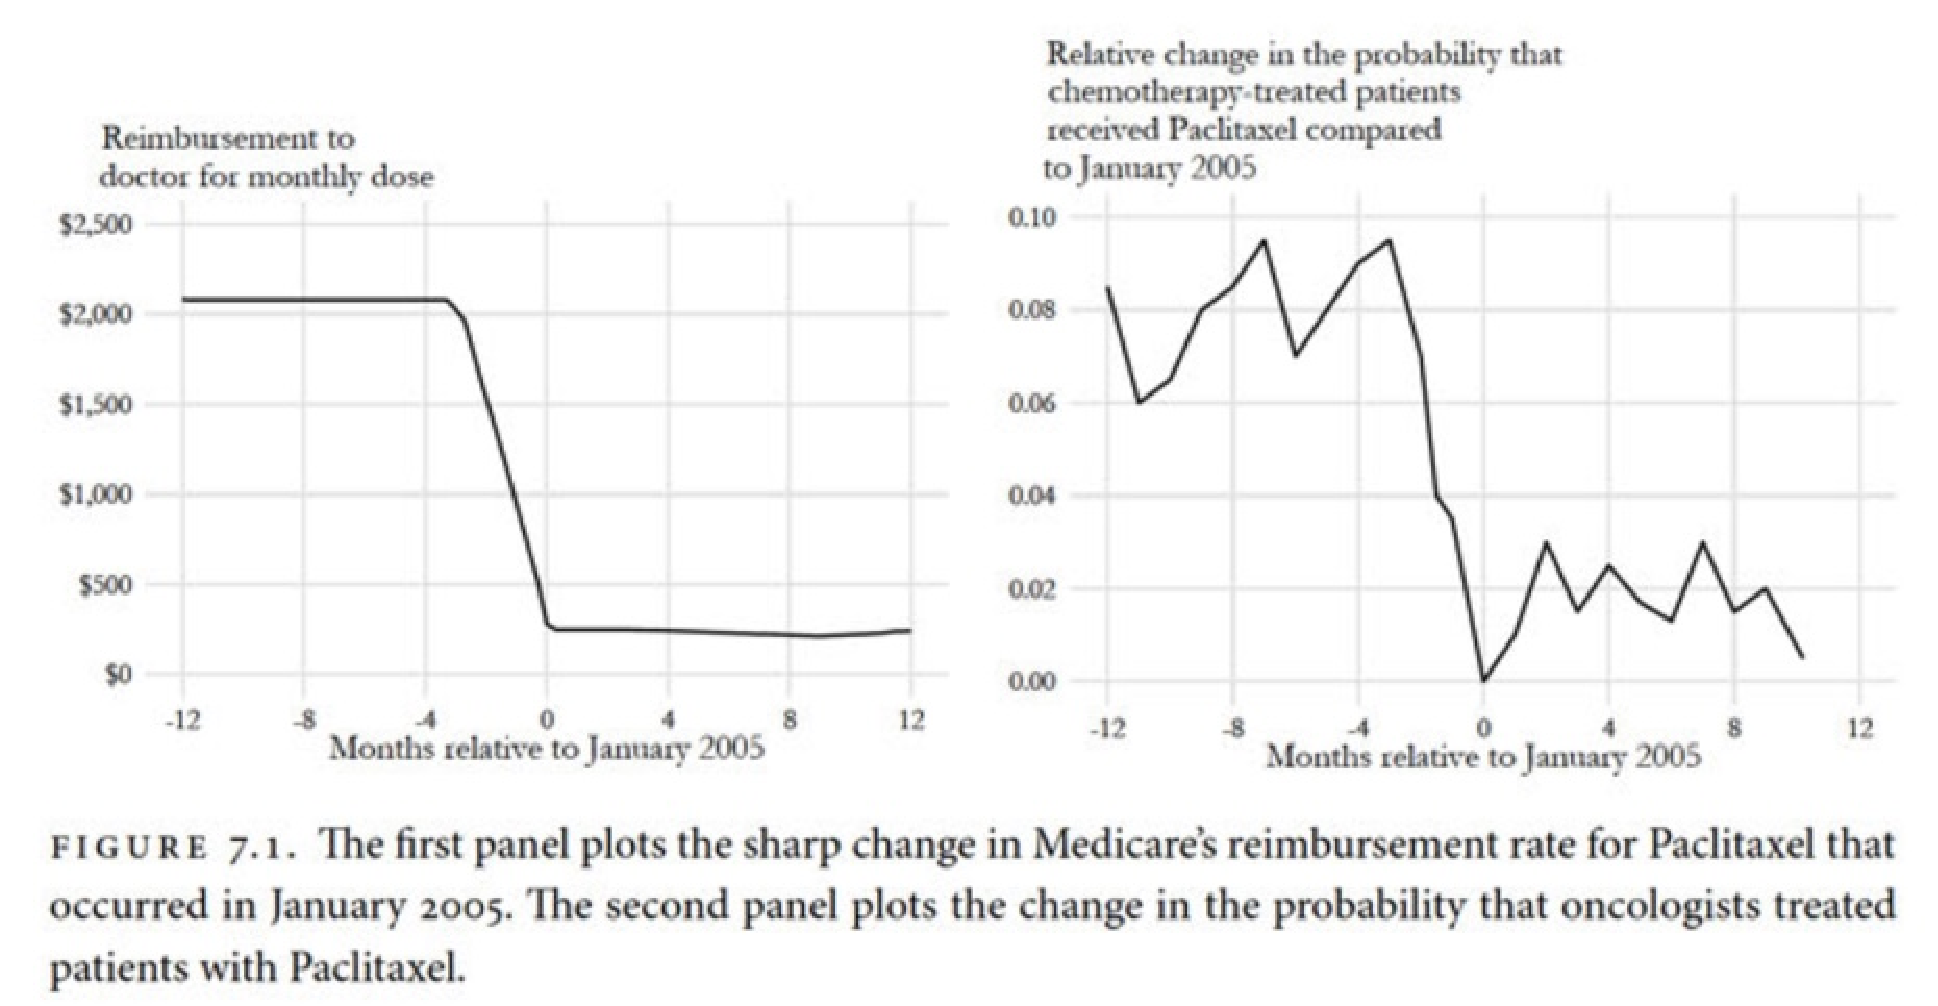
\includegraphics[height=0.75\textheight]{input/GrossNoto_fig7_1.pdf}
    \end{center}

    {\tiny Source: \textit{Better Health Economics} by Tal Gross and Matthew Notowidigdo, chapter 7.}

\end{frame}
%---------------------------------------------------------------------
% \begin{frame}{Large variation in physician earnings across regions}

    
%     \begin{center}
%         \only<1>{
%             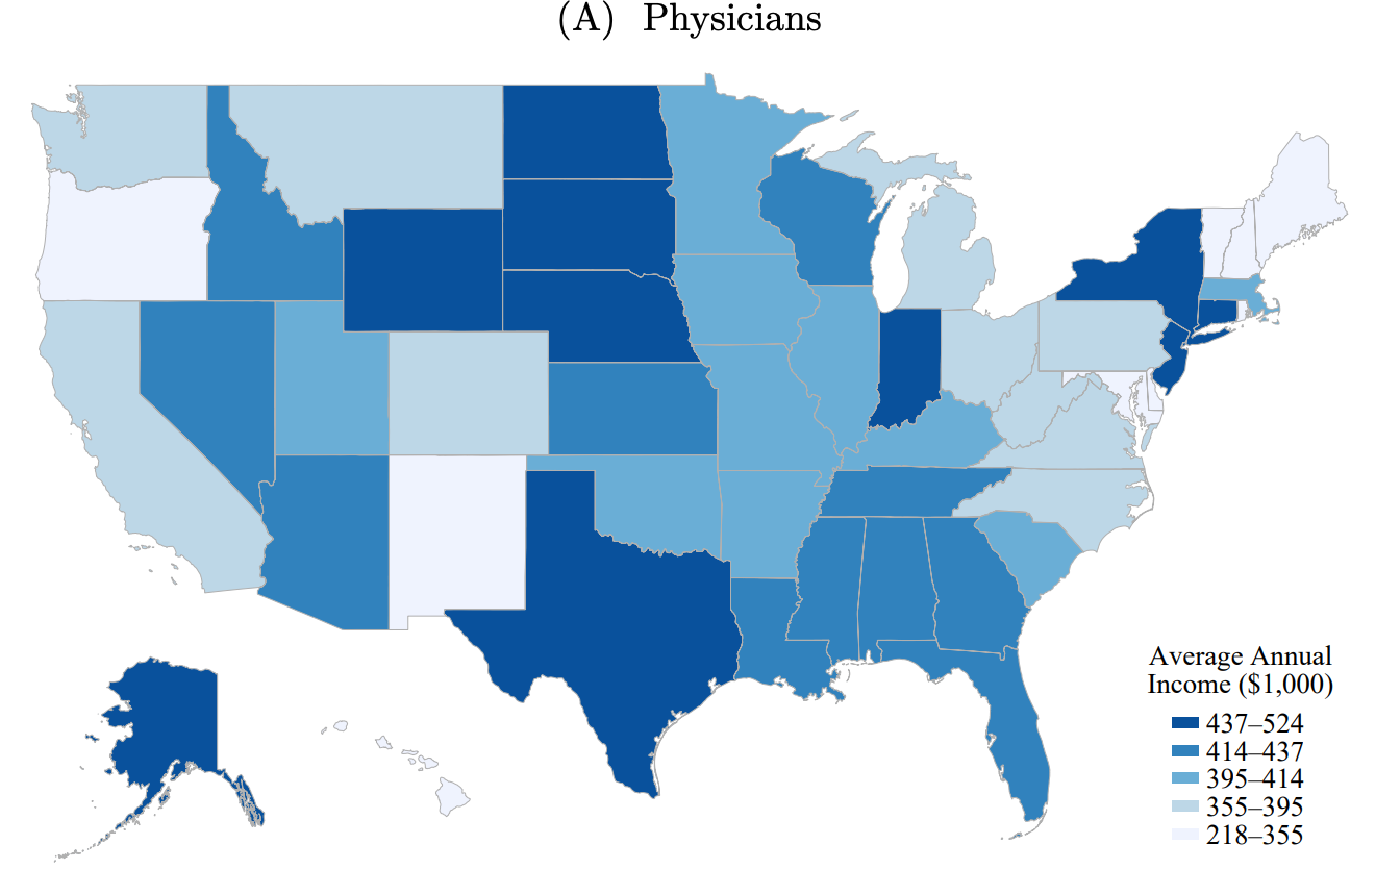
\includegraphics[height=0.8\textheight]{input/Gottlieb_mapphysearnings.pdf}
%         }
%         \only<2>{
%             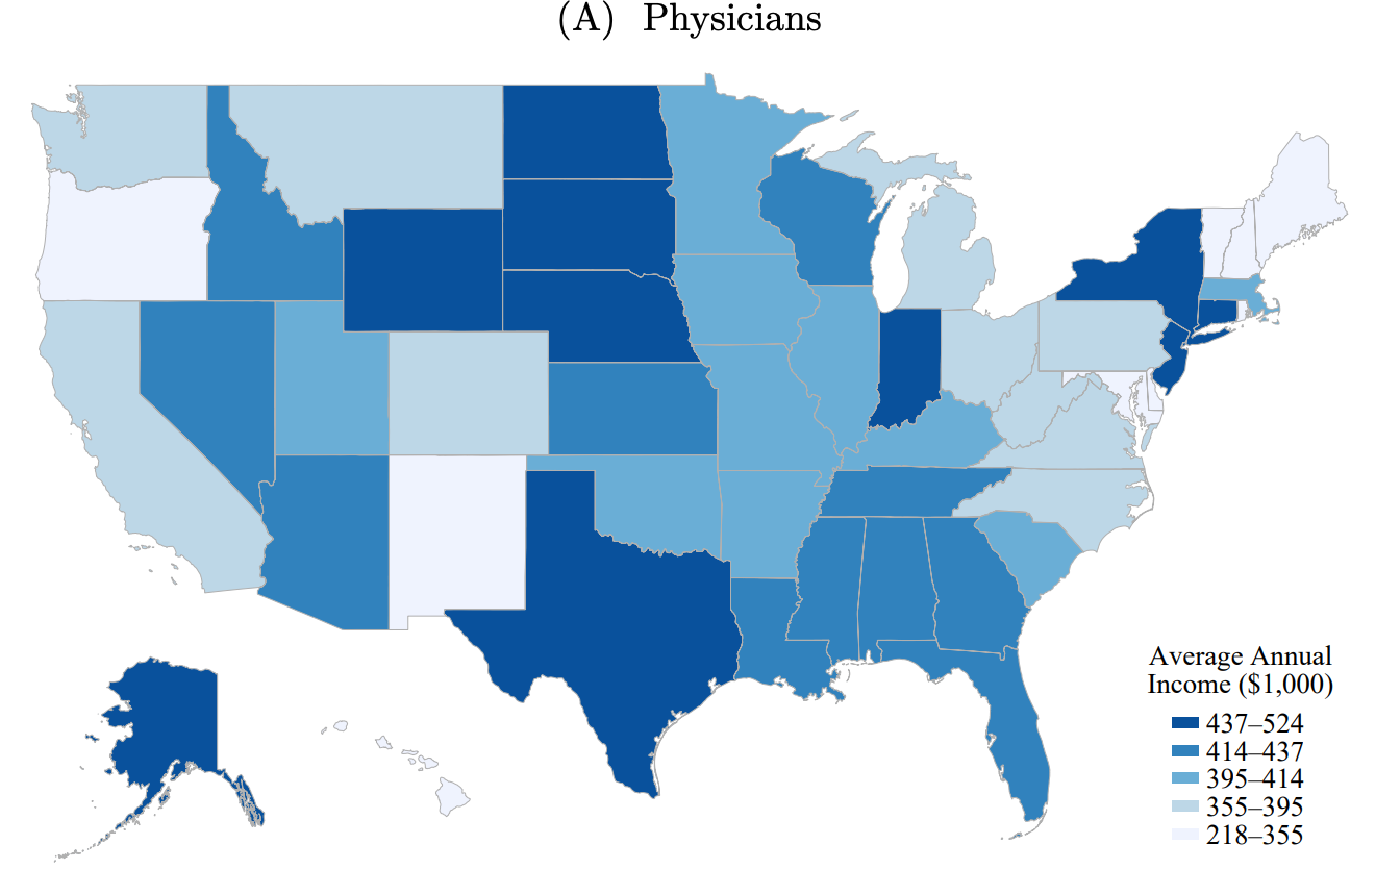
\includegraphics[height=0.5\textheight]{input/Gottlieb_mapphysearnings.pdf}
%             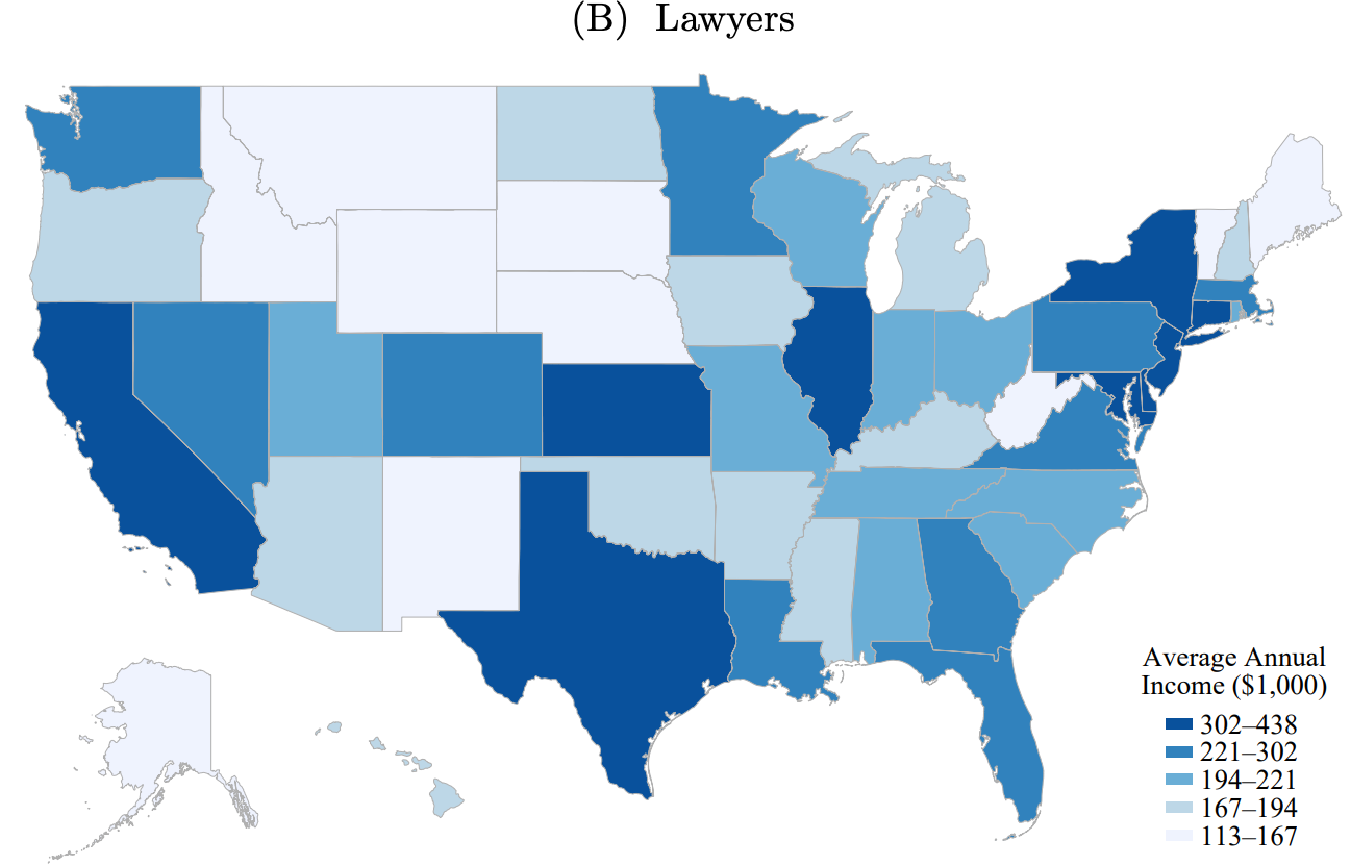
\includegraphics[height=0.5\textheight]{input/Gottlieb_maplawyerearnings.pdf}
%         }
%     \end{center}
    
%     \footnotesize Gottlieb, Polyakova, Rinz, Shiplett, and Udalova (2025)
% \end{frame}
% %---------------------------------------------------------------------
% \begin{frame}{Physician earnings across specialties: hours worked and training}

%     \begin{center}
%         \only<1>{
%             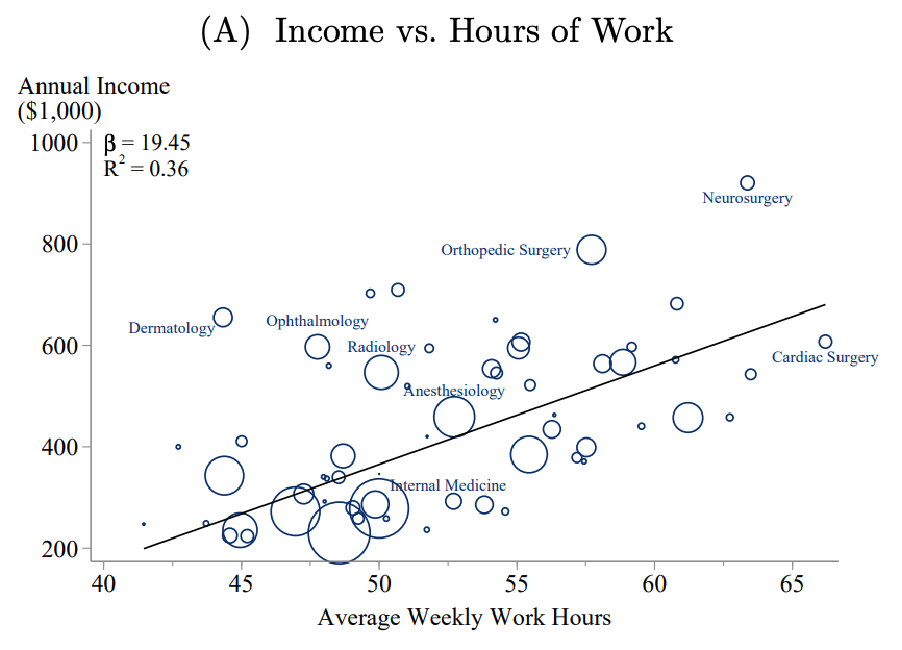
\includegraphics[height=0.8\textheight]{input/Gottlieb_incometohours.pdf}
%         }
%         \only<2>{
%             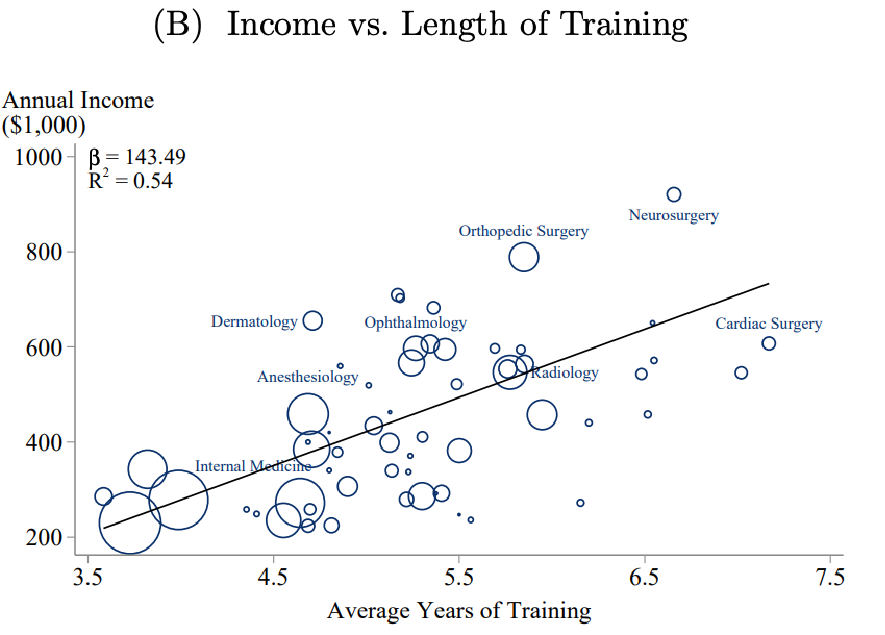
\includegraphics[height=0.8\textheight]{input/Gottlieb_incometotraining.pdf}
%         }
%     \end{center}
    
%     \footnotesize Gottlieb, Polyakova, Rinz, Shiplett, and Udalova (2025)
% \end{frame}
% %---------------------------------------------------------------------
\begin{frame}{Navigating the healthcare system is tricky...}

    \begin{center}
        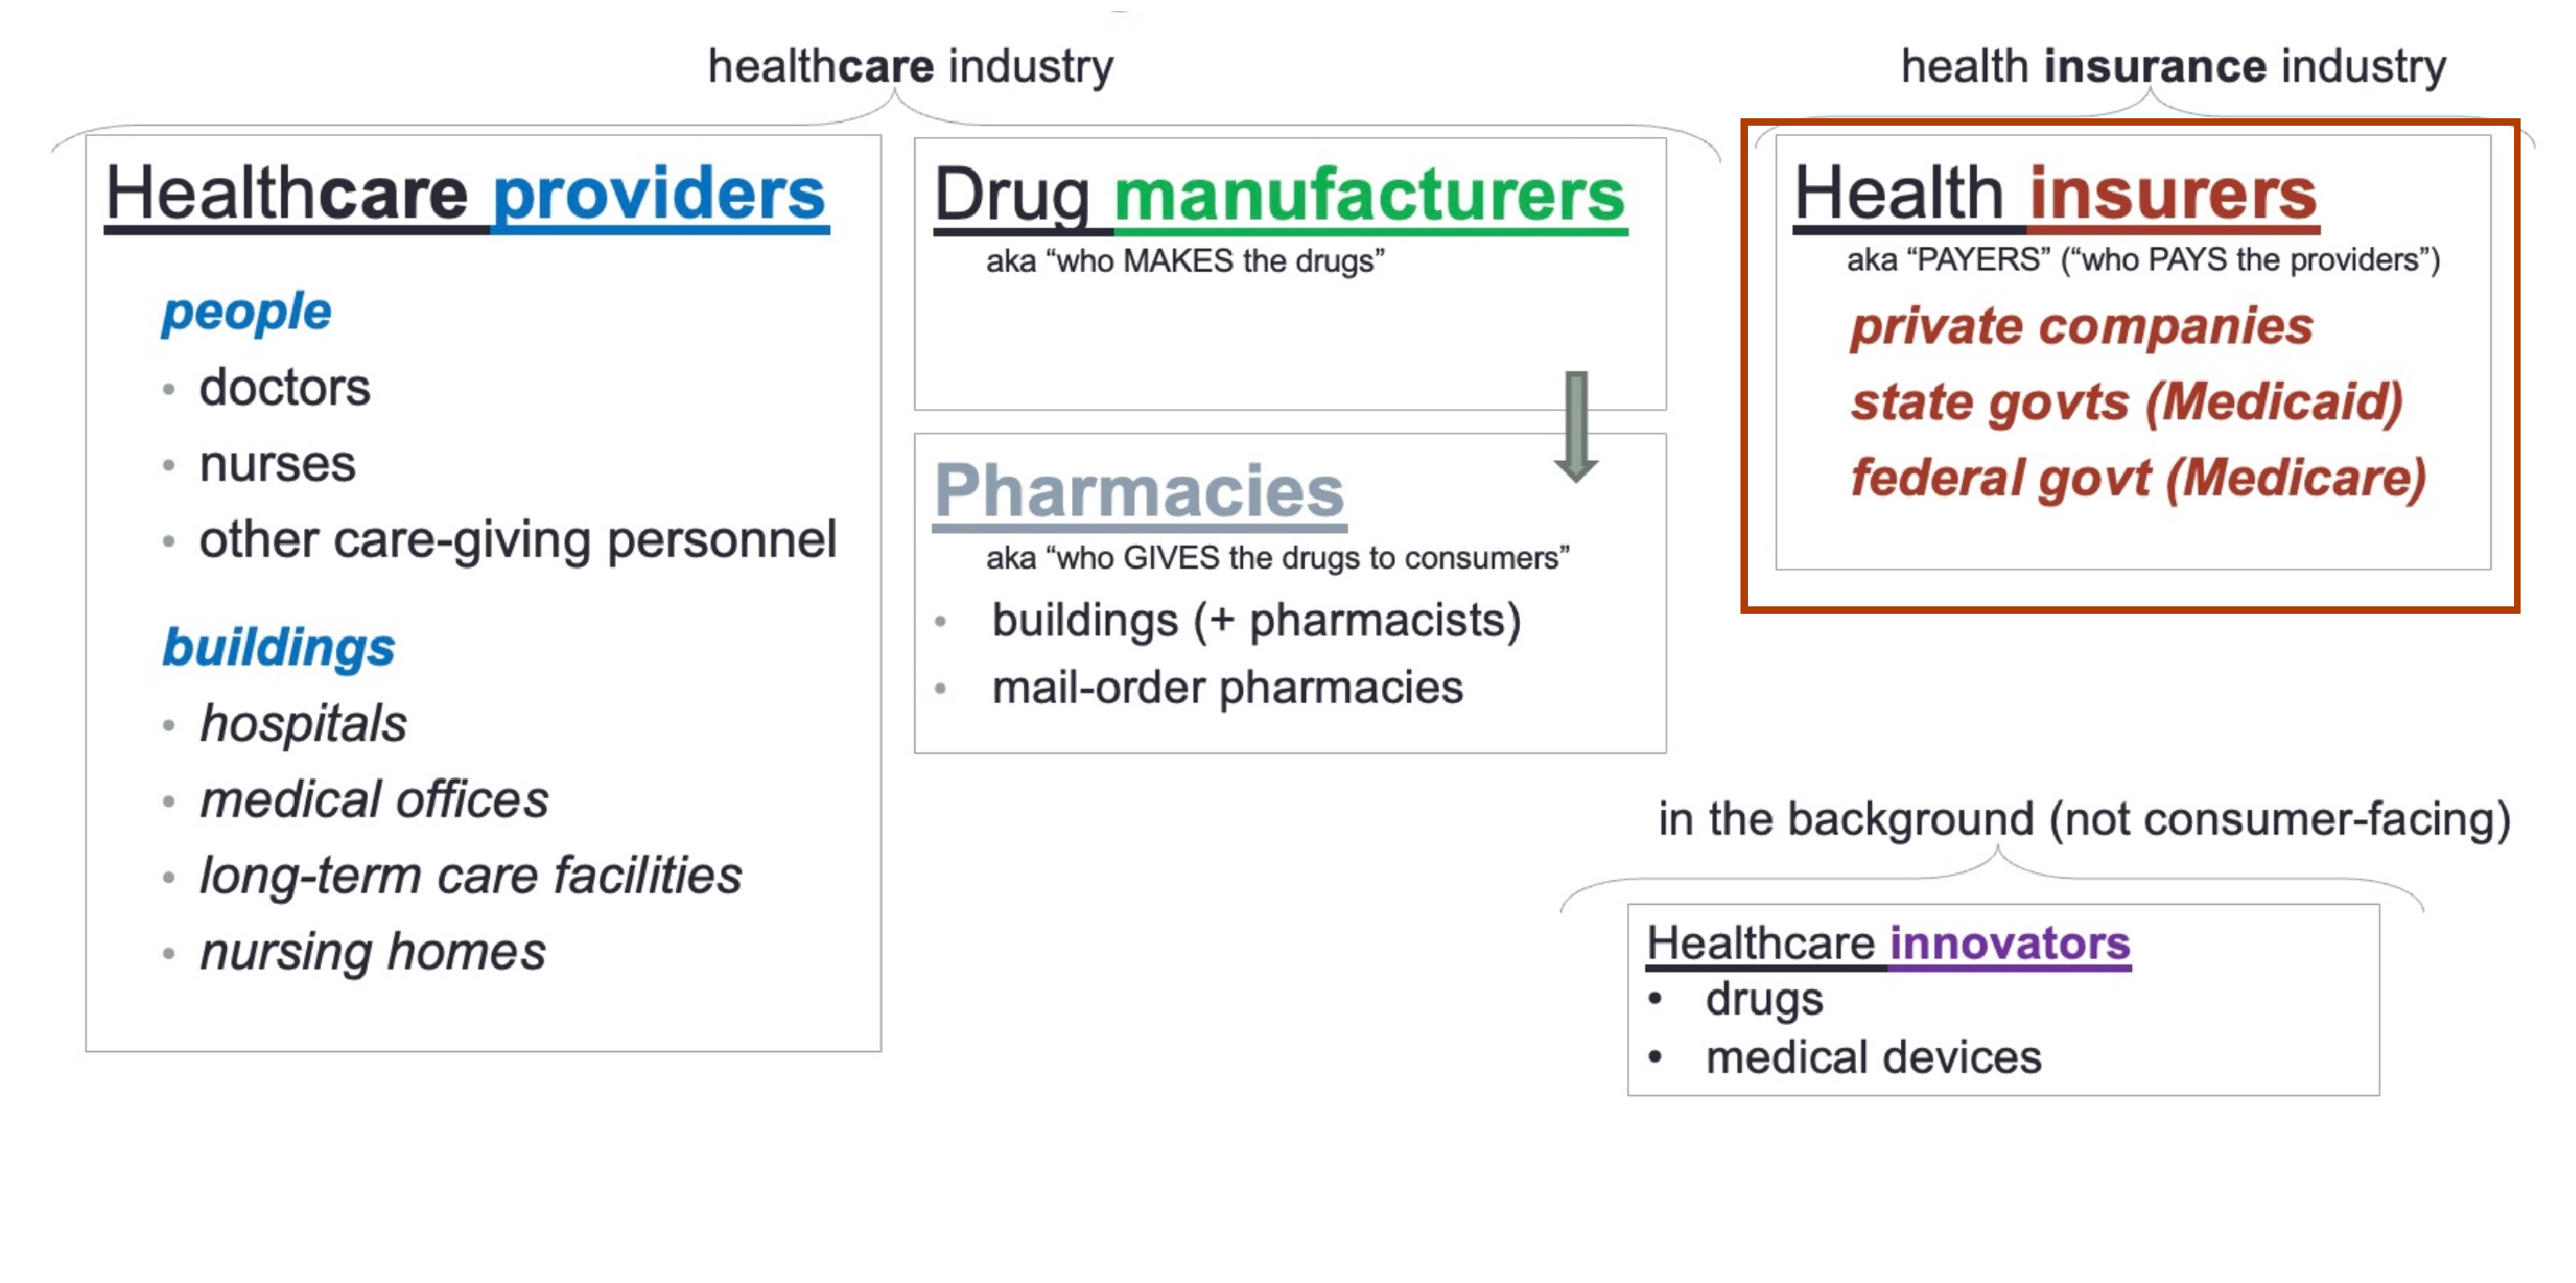
\includegraphics[height=0.85\textheight]{input/marone_UShealthcaresystem.pdf}
    \end{center}

\end{frame}
%---------------------------------------------------------------------
\begin{frame}{... and trickier}

    \begin{center}
        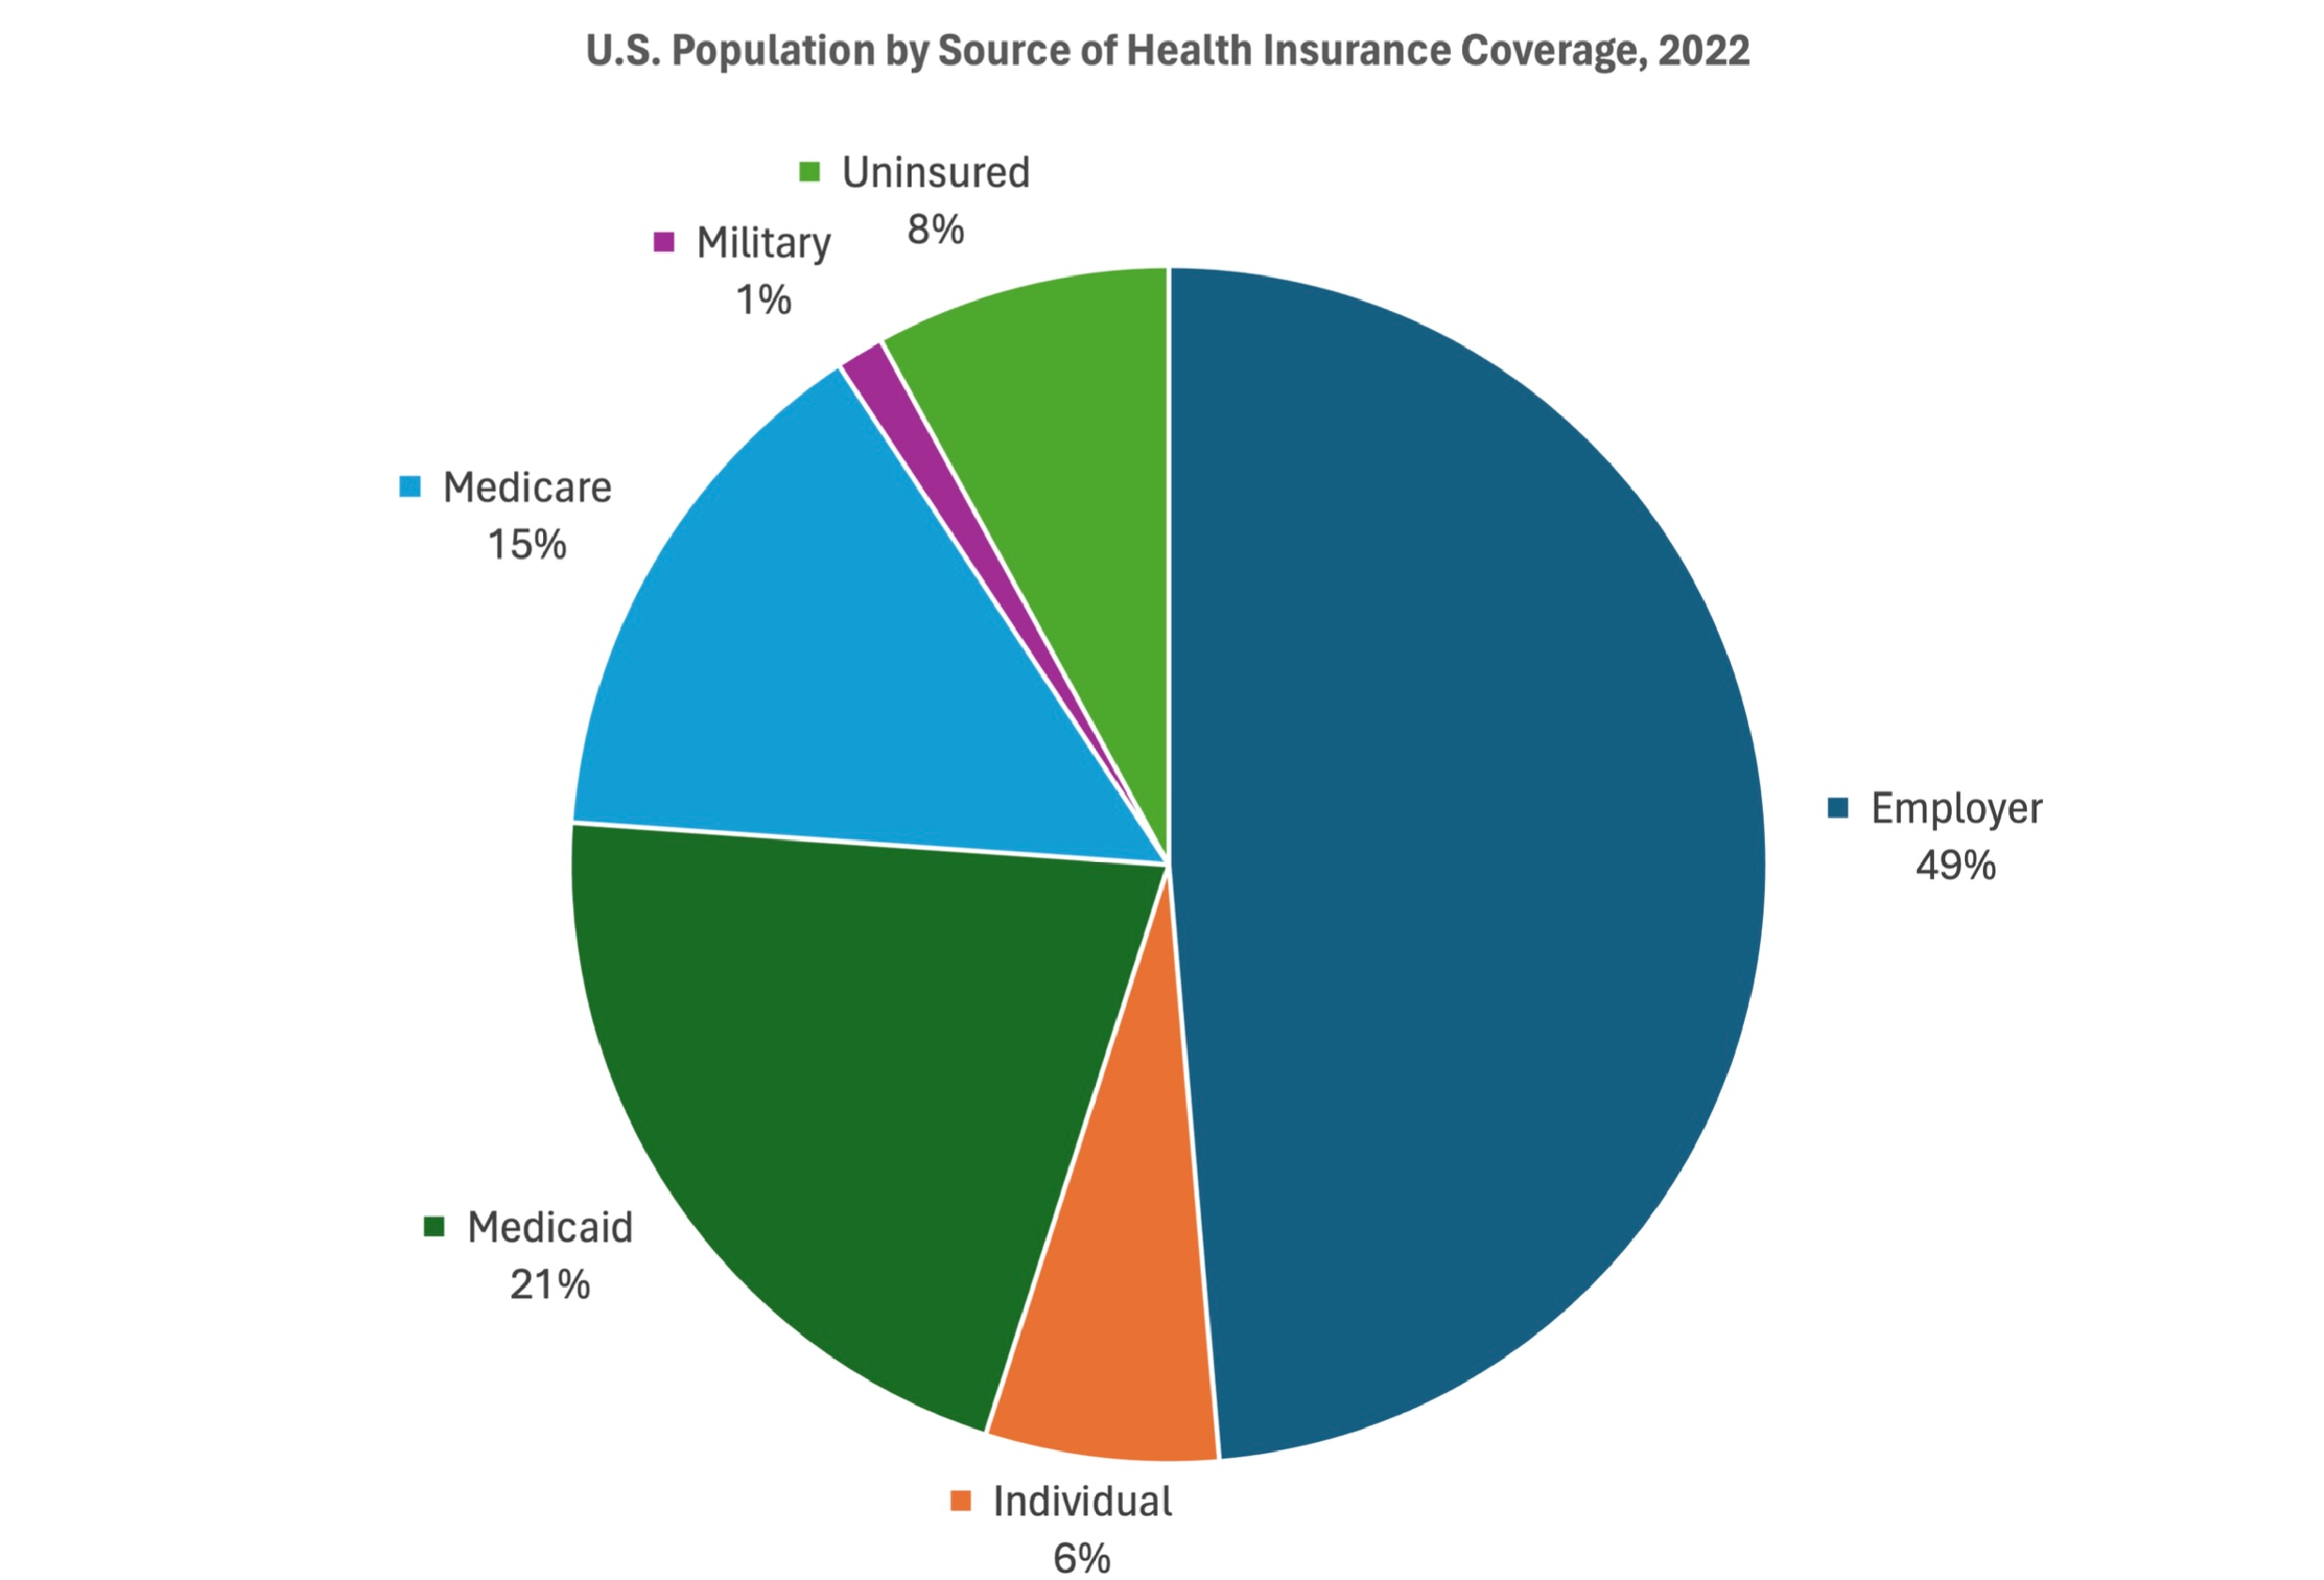
\includegraphics[height=0.85\textheight]{input/marone_sourceinsurance.pdf}
    \end{center}
    % Check sources, probably KSS
\end{frame}
%---------------------------------------------------------------------
\begin{frame}{An insurance plan for employees at BU}

    \begin{center}
        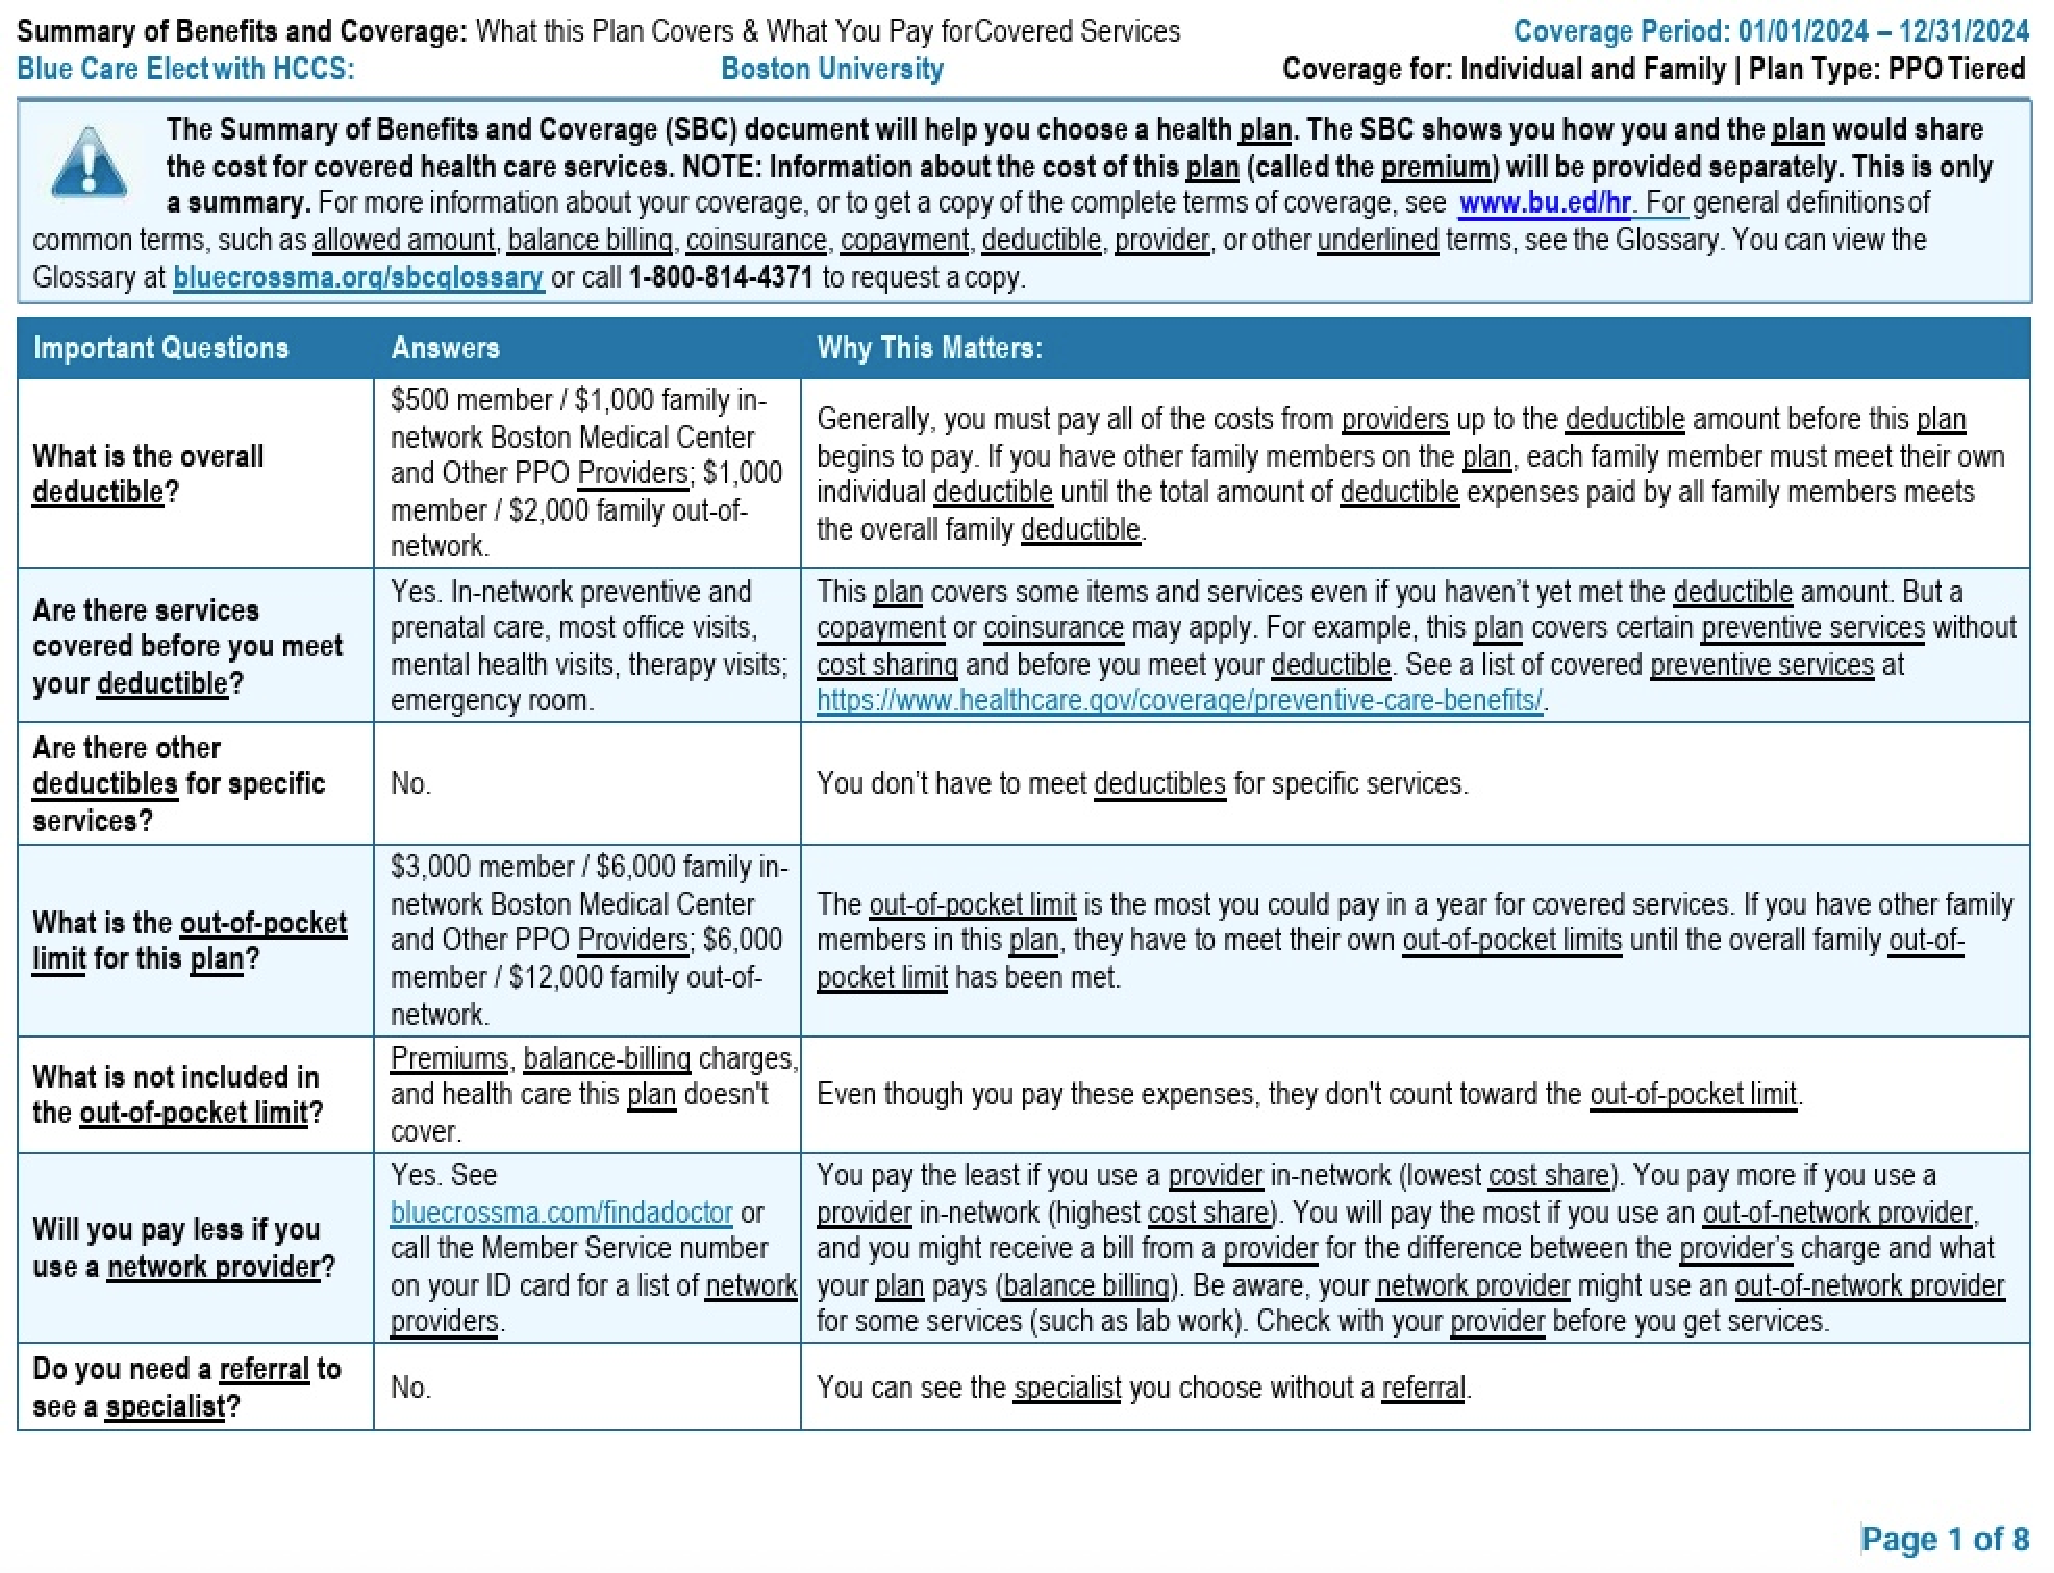
\includegraphics[height=0.95\textheight]{input/examplesummarybenefits_bu24.pdf}
    \end{center}
\end{frame}
%---------------------------------------------------------------------
\begin{frame}{When do we meet?}

    \begin{itemize}
        \item \newbold{Class}\\
        Twice a week: Tuesdays \& Thursdays 9:30am-10:45am in 685-725 Comm Ave CAS 226.
        \vspace{3mm}

        \item \newbold{Office hours}\\
        Chloe Song (your TA): Wednesdays 3-5 PM in SSW B03A.\\
        Pauline Mourot (me): Thursdays 1:30-3:30PM in SSW 545.
    \end{itemize}
\end{frame}
%---------------------------------------------------------------------
\begin{frame}{Format of the course}

    \begin{itemize}
        % \item Some lectures will involve a \newbold{worksheet}
        % \begin{itemize}
        %     \item Posted on Blackboard before the class
        %     \item We will discuss and go through them in class
        %     \item Solutions will be posted when we do not have time to go through them in class
        % \end{itemize}
        % \vspace{3mm}

        \item We will have \newbold{problem sets}, fully graded
        \begin{itemize}
            \item There will be \textbf{five} of them
            \item Will drop the lowest grade of the five
        \end{itemize}
        \vspace{3mm}

        \item 3 \newbold{exams}
        \begin{itemize}
            \item Midterm 1: Thursday, February 19th.
            \item Midterm 2: Thursday, April 2nd.
            \item Final: TBD.
        \end{itemize}
    \end{itemize}
\end{frame}
%---------------------------------------------------------------------
\begin{frame}{Course material (completely optional)}

    \begin{columns}[T]   % T = top alignment
        % ---------------- LEFT COLUMN ----------------
        \begin{column}{0.8\textwidth}
            \begin{itemize}
                \item More standard textbook: \\
                \textit{Health Economics} by Jay Bhattacharya, Timothy Hyde, and Peter Tu
    
                \vspace{6mm}
    
                \item More conversational reference: \\
                \textit{Better Health Economics} by Tal Gross and Matthew Notowidigdo
            \end{itemize}
    
            \vspace{4mm}
            $\implies$ These references are \newbold{optional}. \\
            Lectures and assigned readings will cover \newbold{all required} course material.
        \end{column}
    
        % ---------------- RIGHT COLUMN ----------------
        \begin{column}{0.2\textwidth}
            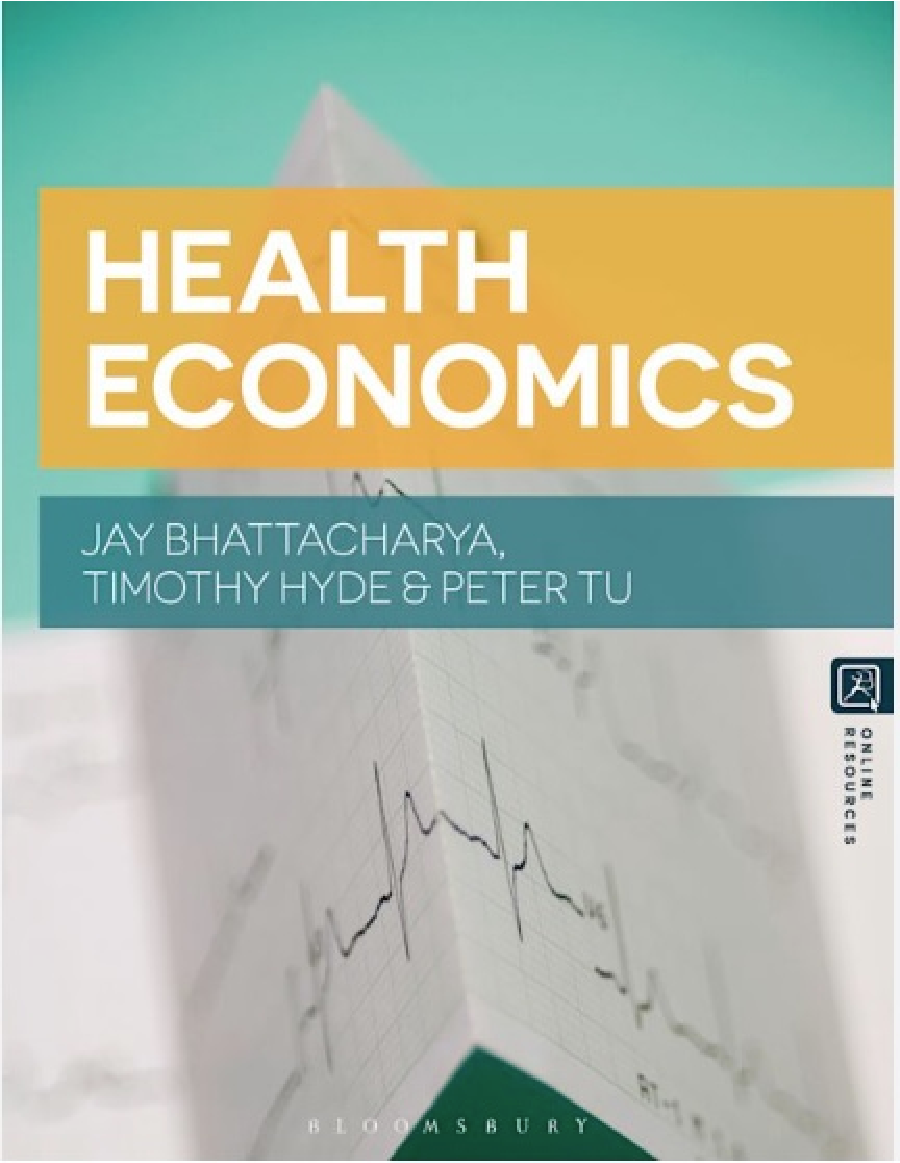
\includegraphics[width=0.7\textwidth]{input/textbook_battacharya.pdf}
    
            \vspace{4mm}
    
            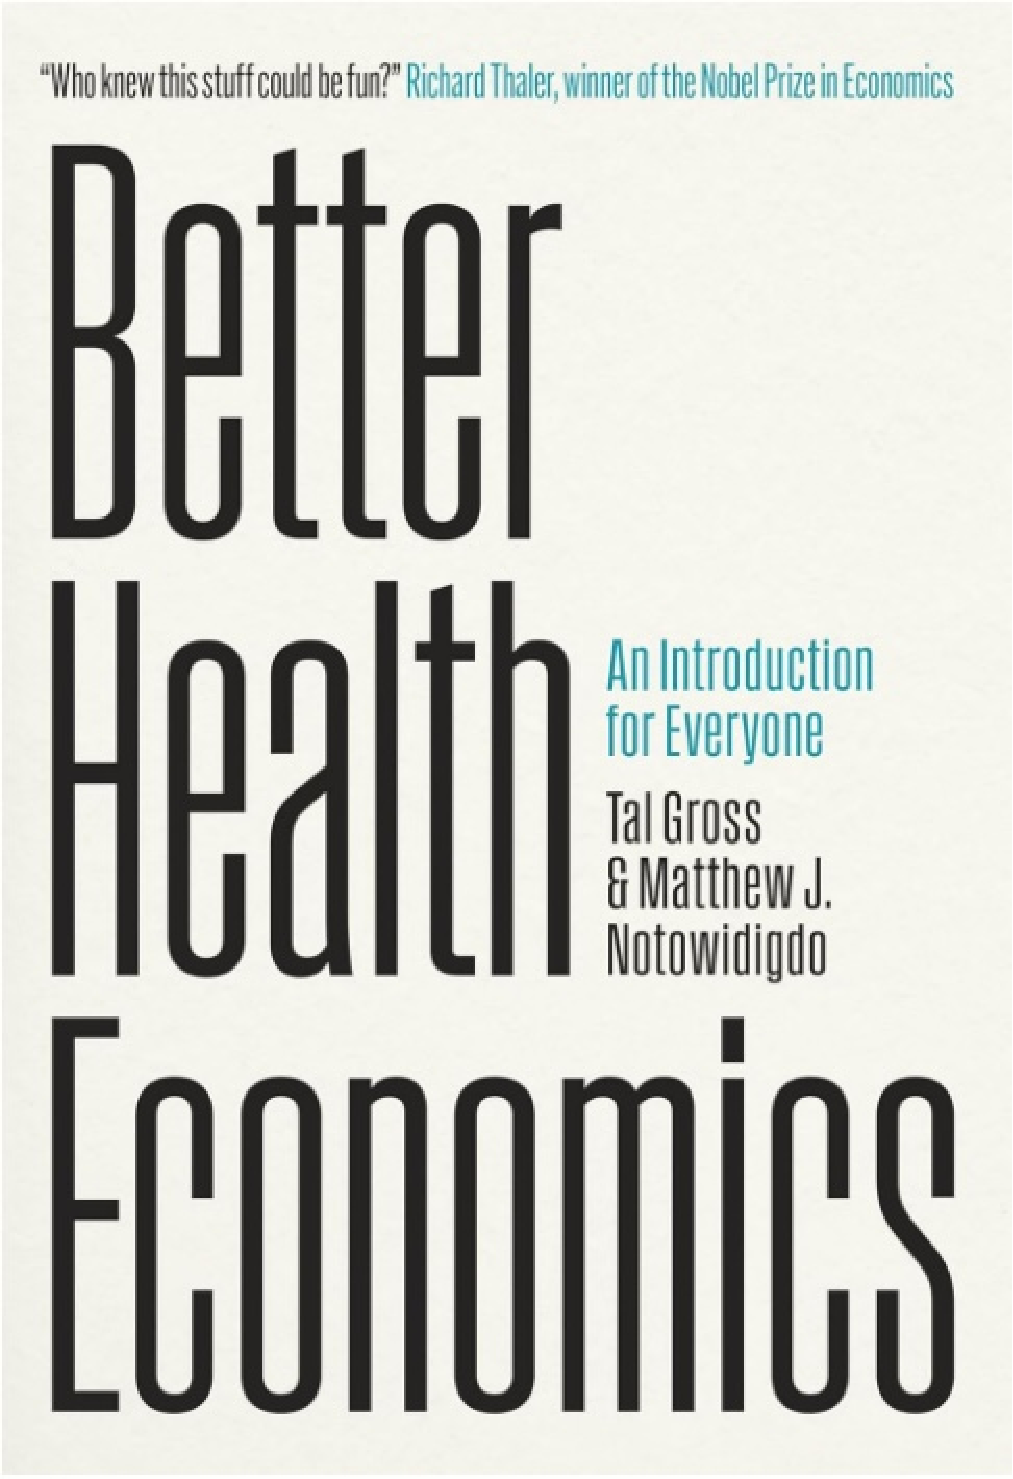
\includegraphics[width=0.7\textwidth]{input/textbook_grossnoto.pdf}
        \end{column}
    \end{columns}

\end{frame}
%---------------------------------------------------------------------
\begin{frame}{Expectations}

    \begin{itemize}
        \item Read the syllabus. This is your responsibility.

        \item Drop the course now if you cannot make the exam dates

        \item Keep up with the course content
        \begin{itemize}
            \item Complete readings before class
            \item Check understanding of covered material during class
            \item Practice by completing the problem sets, learn from your mistakes using the detailed solutions
            \item Come to office hours to ask questions
        \end{itemize}
    \end{itemize}
    \vspace{3mm}

    \textbf{Important}: if you need special accomodation for exams, please let me know by February 3rd, 2026.
\end{frame}
%---------------------------------------------------------------------
\begin{frame}{}

    {\Large \textcolor{maroon}{Let's take a look at the syllabus}}
    
\end{frame}
%---------------------------------------------------------------------  